\documentclass[1p]{elsarticle_modified}
%\bibliographystyle{elsarticle-num}

%\usepackage[colorlinks]{hyperref}
%\usepackage{abbrmath_seonhwa} %\Abb, \Ascr, \Acal ,\Abf, \Afrak
\usepackage{amsfonts}
\usepackage{amssymb}
\usepackage{amsmath}
\usepackage{amsthm}
\usepackage{scalefnt}
\usepackage{amsbsy}
\usepackage{kotex}
\usepackage{caption}
\usepackage{subfig}
\usepackage{color}
\usepackage{graphicx}
\usepackage{xcolor} %% white, black, red, green, blue, cyan, magenta, yellow
\usepackage{float}
\usepackage{setspace}
\usepackage{hyperref}

\usepackage{tikz}
\usetikzlibrary{arrows}

\usepackage{multirow}
\usepackage{array} % fixed length table
\usepackage{hhline}

%%%%%%%%%%%%%%%%%%%%%
\makeatletter
\renewcommand*\env@matrix[1][\arraystretch]{%
	\edef\arraystretch{#1}%
	\hskip -\arraycolsep
	\let\@ifnextchar\new@ifnextchar
	\array{*\c@MaxMatrixCols c}}
\makeatother %https://tex.stackexchange.com/questions/14071/how-can-i-increase-the-line-spacing-in-a-matrix
%%%%%%%%%%%%%%%

\usepackage[normalem]{ulem}

\newcommand{\msout}[1]{\ifmmode\text{\sout{\ensuremath{#1}}}\else\sout{#1}\fi}
%SOURCE: \msout is \stkout macro in https://tex.stackexchange.com/questions/20609/strikeout-in-math-mode

\newcommand{\cancel}[1]{
	\ifmmode
	{\color{red}\msout{#1}}
	\else
	{\color{red}\sout{#1}}
	\fi
}

\newcommand{\add}[1]{
	{\color{blue}\uwave{#1}}
}

\newcommand{\replace}[2]{
	\ifmmode
	{\color{red}\msout{#1}}{\color{blue}\uwave{#2}}
	\else
	{\color{red}\sout{#1}}{\color{blue}\uwave{#2}}
	\fi
}

\newcommand{\Sol}{\mathcal{S}} %segment
\newcommand{\D}{D} %diagram
\newcommand{\A}{\mathcal{A}} %arc


%%%%%%%%%%%%%%%%%%%%%%%%%%%%%5 test

\def\sl{\operatorname{\textup{SL}}(2,\Cbb)}
\def\psl{\operatorname{\textup{PSL}}(2,\Cbb)}
\def\quan{\mkern 1mu \triangleright \mkern 1mu}

\theoremstyle{definition}
\newtheorem{thm}{Theorem}[section]
\newtheorem{prop}[thm]{Proposition}
\newtheorem{lem}[thm]{Lemma}
\newtheorem{ques}[thm]{Question}
\newtheorem{cor}[thm]{Corollary}
\newtheorem{defn}[thm]{Definition}
\newtheorem{exam}[thm]{Example}
\newtheorem{rmk}[thm]{Remark}
\newtheorem{alg}[thm]{Algorithm}

\newcommand{\I}{\sqrt{-1}}
\begin{document}

%\begin{frontmatter}
%
%\title{Boundary parabolic representations of knots up to 8 crossings}
%
%%% Group authors per affiliation:
%\author{Yunhi Cho} 
%\address{Department of Mathematics, University of Seoul, Seoul, Korea}
%\ead{yhcho@uos.ac.kr}
%
%
%\author{Seonhwa Kim} %\fnref{s_kim}}
%\address{Center for Geometry and Physics, Institute for Basic Science, Pohang, 37673, Korea}
%\ead{ryeona17@ibs.re.kr}
%
%\author{Hyuk Kim}
%\address{Department of Mathematical Sciences, Seoul National University, Seoul 08826, Korea}
%\ead{hyukkim@snu.ac.kr}
%
%\author{Seokbeom Yoon}
%\address{Department of Mathematical Sciences, Seoul National University, Seoul, 08826,  Korea}
%\ead{sbyoon15@snu.ac.kr}
%
%\begin{abstract}
%We find all boundary parabolic representation of knots up to 8 crossings.
%
%\end{abstract}
%\begin{keyword}
%    \MSC[2010] 57M25 
%\end{keyword}
%
%\end{frontmatter}

%\linenumbers
%\tableofcontents
%
\newcommand\colored[1]{\textcolor{white}{\rule[-0.35ex]{0.8em}{1.4ex}}\kern-0.8em\color{red} #1}%
%\newcommand\colored[1]{\textcolor{white}{ #1}\kern-2.17ex	\textcolor{white}{ #1}\kern-1.81ex	\textcolor{white}{ #1}\kern-2.15ex\color{red}#1	}

{\Large $\underline{12n_{0174}~(K12n_{0174})}$}

\setlength{\tabcolsep}{10pt}
\renewcommand{\arraystretch}{1.6}
\vspace{1cm}\begin{tabular}{m{100pt}>{\centering\arraybackslash}m{274pt}}
\multirow{5}{120pt}{
	\centering
	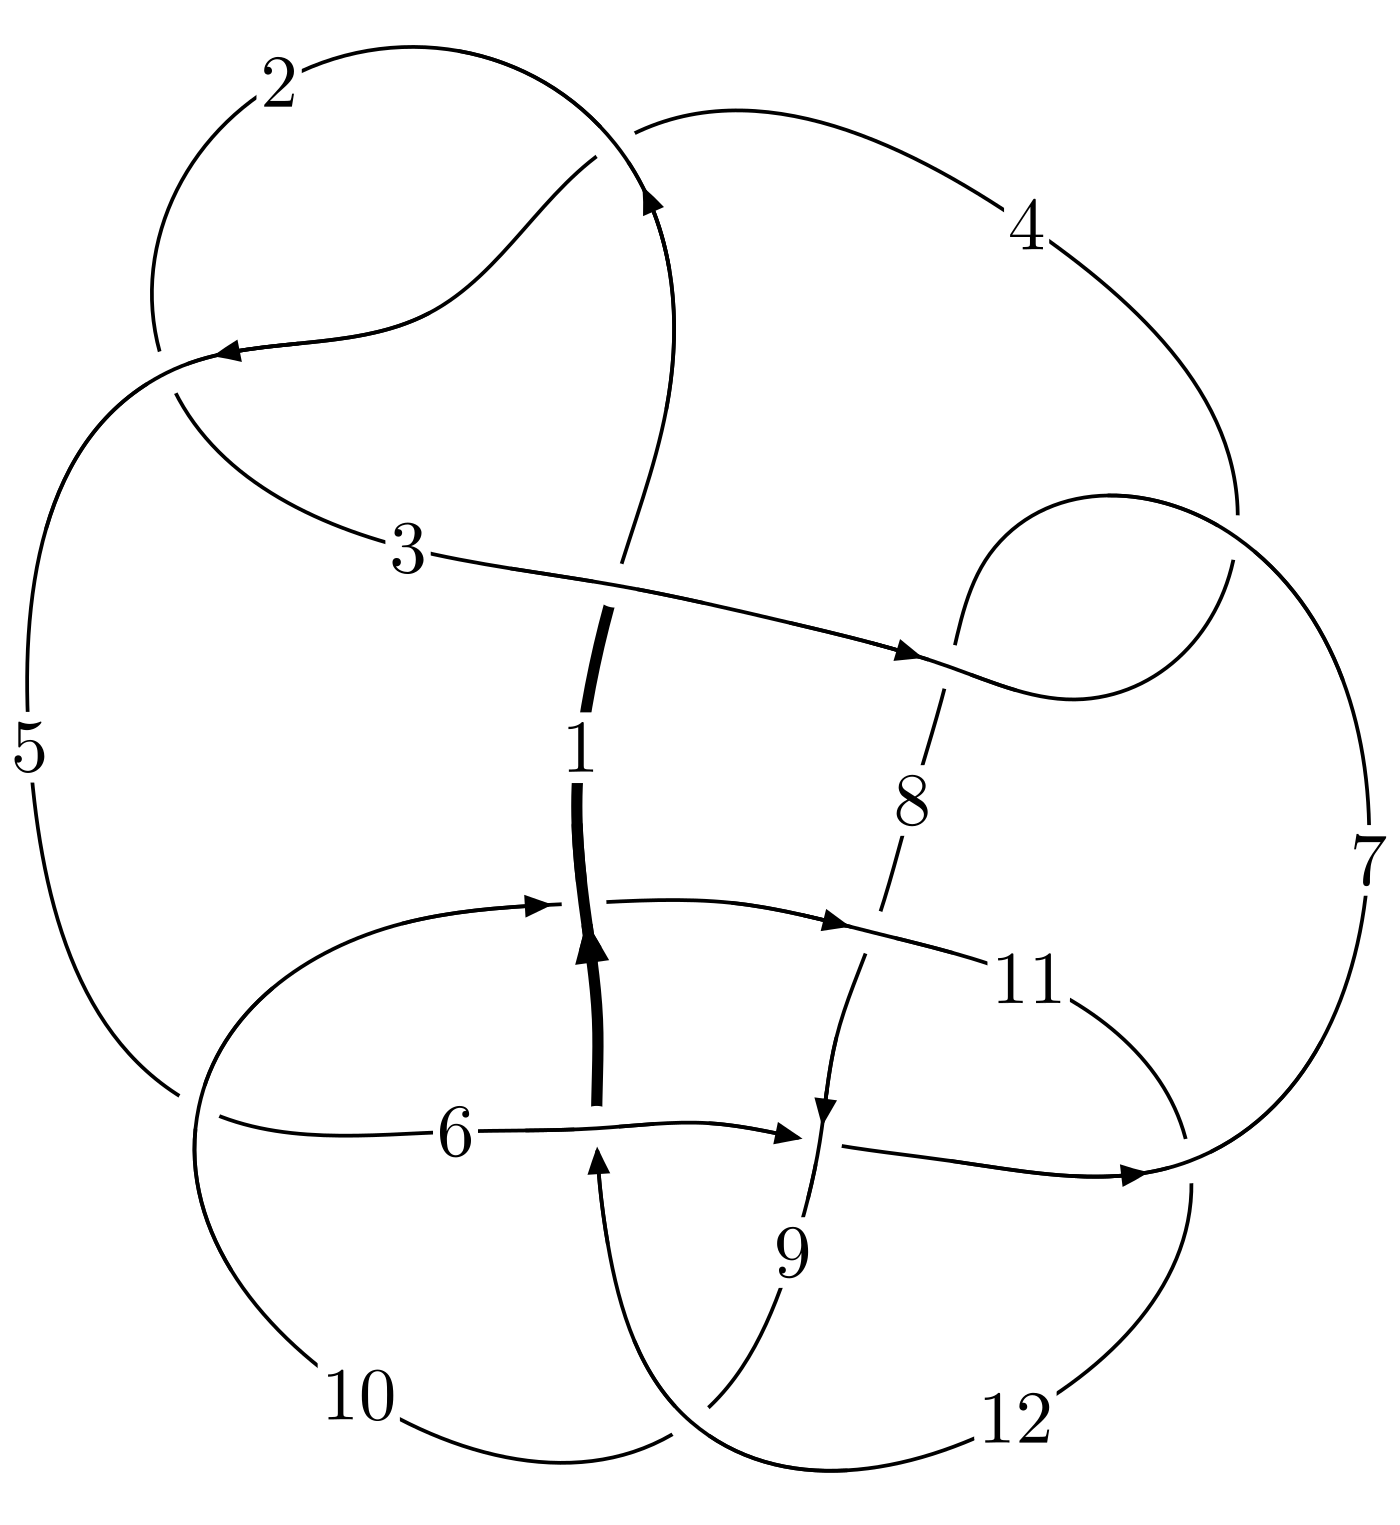
\includegraphics[width=112pt]{../../../GIT/diagram.site/Diagrams/png/2263_12n_0174.png}\\
\ \ \ A knot diagram\footnotemark}&
\allowdisplaybreaks
\textbf{Linearized knot diagam} \\
\cline{2-2}
 &
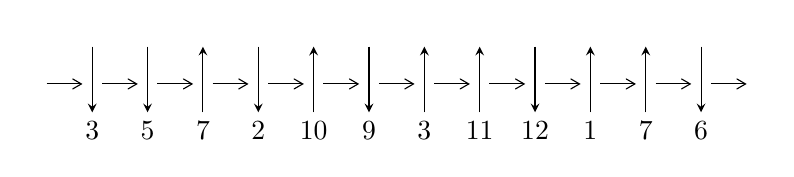
\begin{tikzpicture}[x=20pt, y=17pt]
	% nodes
	\node (C0) at (0, 0) {};
	\node (C1) at (1, 0) {};
	\node (C1U) at (1, +1) {};
	\node (C1D) at (1, -1) {3};

	\node (C2) at (2, 0) {};
	\node (C2U) at (2, +1) {};
	\node (C2D) at (2, -1) {5};

	\node (C3) at (3, 0) {};
	\node (C3U) at (3, +1) {};
	\node (C3D) at (3, -1) {7};

	\node (C4) at (4, 0) {};
	\node (C4U) at (4, +1) {};
	\node (C4D) at (4, -1) {2};

	\node (C5) at (5, 0) {};
	\node (C5U) at (5, +1) {};
	\node (C5D) at (5, -1) {10};

	\node (C6) at (6, 0) {};
	\node (C6U) at (6, +1) {};
	\node (C6D) at (6, -1) {9};

	\node (C7) at (7, 0) {};
	\node (C7U) at (7, +1) {};
	\node (C7D) at (7, -1) {3};

	\node (C8) at (8, 0) {};
	\node (C8U) at (8, +1) {};
	\node (C8D) at (8, -1) {11};

	\node (C9) at (9, 0) {};
	\node (C9U) at (9, +1) {};
	\node (C9D) at (9, -1) {12};

	\node (C10) at (10, 0) {};
	\node (C10U) at (10, +1) {};
	\node (C10D) at (10, -1) {1};

	\node (C11) at (11, 0) {};
	\node (C11U) at (11, +1) {};
	\node (C11D) at (11, -1) {7};

	\node (C12) at (12, 0) {};
	\node (C12U) at (12, +1) {};
	\node (C12D) at (12, -1) {6};
	\node (C13) at (13, 0) {};

	% arrows
	\draw[->,>={angle 60}]
	(C0) edge (C1) (C1) edge (C2) (C2) edge (C3) (C3) edge (C4) (C4) edge (C5) (C5) edge (C6) (C6) edge (C7) (C7) edge (C8) (C8) edge (C9) (C9) edge (C10) (C10) edge (C11) (C11) edge (C12) (C12) edge (C13) ;	\draw[->,>=stealth]
	(C1U) edge (C1D) (C2U) edge (C2D) (C3D) edge (C3U) (C4U) edge (C4D) (C5D) edge (C5U) (C6U) edge (C6D) (C7D) edge (C7U) (C8D) edge (C8U) (C9U) edge (C9D) (C10D) edge (C10U) (C11D) edge (C11U) (C12U) edge (C12D) ;
	\end{tikzpicture} \\
\hhline{~~} \\& 
\textbf{Solving Sequence} \\ \cline{2-2} 
 &
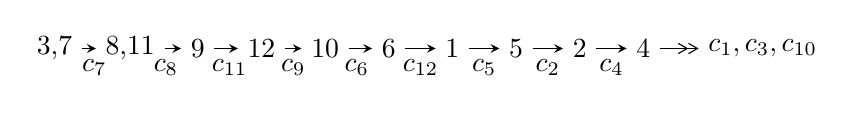
\begin{tikzpicture}[x=23pt, y=7pt]
	% node
	\node (A0) at (-1/8, 0) {3,7};
	\node (A1) at (17/16, 0) {8,11};
	\node (A2) at (17/8, 0) {9};
	\node (A3) at (25/8, 0) {12};
	\node (A4) at (33/8, 0) {10};
	\node (A5) at (41/8, 0) {6};
	\node (A6) at (49/8, 0) {1};
	\node (A7) at (57/8, 0) {5};
	\node (A8) at (65/8, 0) {2};
	\node (A9) at (73/8, 0) {4};
	\node (C1) at (1/2, -1) {$c_{7}$};
	\node (C2) at (13/8, -1) {$c_{8}$};
	\node (C3) at (21/8, -1) {$c_{11}$};
	\node (C4) at (29/8, -1) {$c_{9}$};
	\node (C5) at (37/8, -1) {$c_{6}$};
	\node (C6) at (45/8, -1) {$c_{12}$};
	\node (C7) at (53/8, -1) {$c_{5}$};
	\node (C8) at (61/8, -1) {$c_{2}$};
	\node (C9) at (69/8, -1) {$c_{4}$};
	\node (A10) at (11, 0) {$c_{1},c_{3},c_{10}$};

	% edge
	\draw[->,>=stealth]	
	(A0) edge (A1) (A1) edge (A2) (A2) edge (A3) (A3) edge (A4) (A4) edge (A5) (A5) edge (A6) (A6) edge (A7) (A7) edge (A8) (A8) edge (A9) ;
	\draw[->>,>={angle 60}]	
	(A9) edge (A10);
\end{tikzpicture} \\ 

\end{tabular} \\

\footnotetext{
The image of knot diagram is generated by the software ``\textbf{Draw programme}" developed by Andrew Bartholomew(\url{http://www.layer8.co.uk/maths/draw/index.htm\#Running-draw}), where we modified some parts for our purpose(\url{https://github.com/CATsTAILs/LinksPainter}).
}\phantom \\ \newline 
\centering \textbf{Ideals for irreducible components\footnotemark of $X_{\text{par}}$} 
 
\begin{align*}
I^u_{1}&=\langle 
-4.42510\times10^{95} u^{48}-1.67612\times10^{96} u^{47}+\cdots+3.37850\times10^{95} b+3.34034\times10^{97},\\
\phantom{I^u_{1}}&\phantom{= \langle  }3.85868\times10^{98} u^{48}+1.60673\times10^{99} u^{47}+\cdots+4.32448\times10^{97} a-1.18824\times10^{101},\\
\phantom{I^u_{1}}&\phantom{= \langle  }u^{49}+5 u^{48}+\cdots-2656 u-256\rangle \\
I^u_{2}&=\langle 
3.65067\times10^{30} a u^{29}+6.18961\times10^{29} u^{29}+\cdots-4.67430\times10^{31} a+3.01744\times10^{30},\\
\phantom{I^u_{2}}&\phantom{= \langle  }4.65337\times10^{30} a u^{29}+5.16674\times10^{30} u^{29}+\cdots-1.73780\times10^{31} a-4.22817\times10^{31},\;u^{30}-3 u^{29}+\cdots-36 u+8\rangle \\
I^u_{3}&=\langle 
62854845 u^{16}+90595385 u^{15}+\cdots+103426241 b-86148102,\\
\phantom{I^u_{3}}&\phantom{= \langle  }825367762 u^{16}+1637559900 u^{15}+\cdots+103426241 a-116862060,\;u^{17}+2 u^{16}+\cdots+u+1\rangle \\
\\
I^v_{1}&=\langle 
a,\;16 v^3-48 v^2+b+51 v-13,\;4 v^4-13 v^3+16 v^2-7 v+1\rangle \\
I^v_{2}&=\langle 
a,\;b^2- b v+v^2- b+2 v+2,\;v^3+2 v^2+3 v+1\rangle \\
\end{align*}
\raggedright * 5 irreducible components of $\dim_{\mathbb{C}}=0$, with total 136 representations.\\
\footnotetext{All coefficients of polynomials are rational numbers. But the coefficients are sometimes approximated in decimal forms when there is not enough margin.}
\newpage
\renewcommand{\arraystretch}{1}
\centering \section*{I. $I^u_{1}= \langle -4.43\times10^{95} u^{48}-1.68\times10^{96} u^{47}+\cdots+3.38\times10^{95} b+3.34\times10^{97},\;3.86\times10^{98} u^{48}+1.61\times10^{99} u^{47}+\cdots+4.32\times10^{97} a-1.19\times10^{101},\;u^{49}+5 u^{48}+\cdots-2656 u-256 \rangle$}
\flushleft \textbf{(i) Arc colorings}\\
\begin{tabular}{m{7pt} m{180pt} m{7pt} m{180pt} }
\flushright $a_{3}=$&$\begin{pmatrix}0\\u\end{pmatrix}$ \\
\flushright $a_{7}=$&$\begin{pmatrix}1\\0\end{pmatrix}$ \\
\flushright $a_{8}=$&$\begin{pmatrix}1\\- u^2\end{pmatrix}$ \\
\flushright $a_{11}=$&$\begin{pmatrix}-8.92288 u^{48}-37.1542 u^{47}+\cdots+25170.8 u+2747.71\\1.30978 u^{48}+4.96113 u^{47}+\cdots-1531.46 u-98.8705\end{pmatrix}$ \\
\flushright $a_{9}=$&$\begin{pmatrix}-17.4967 u^{48}-72.9082 u^{47}+\cdots+49242.2 u+5362.98\\5.84693 u^{48}+24.9569 u^{47}+\cdots-19011.2 u-2144.77\end{pmatrix}$ \\
\flushright $a_{12}=$&$\begin{pmatrix}-7.61310 u^{48}-32.1931 u^{47}+\cdots+23639.3 u+2648.84\\1.30978 u^{48}+4.96113 u^{47}+\cdots-1531.46 u-98.8705\end{pmatrix}$ \\
\flushright $a_{10}=$&$\begin{pmatrix}0.226092 u^{48}+1.59877 u^{47}+\cdots-3637.18 u-493.367\\2.11651 u^{48}+9.72772 u^{47}+\cdots-10201.7 u-1249.45\end{pmatrix}$ \\
\flushright $a_{6}=$&$\begin{pmatrix}-0.0565490 u^{48}-0.741312 u^{47}+\cdots+2683.08 u+377.332\\-1.10782 u^{48}-5.50733 u^{47}+\cdots+7171.36 u+910.721\end{pmatrix}$ \\
\flushright $a_{1}=$&$\begin{pmatrix}-0.489227 u^{48}-1.92395 u^{47}+\cdots+911.166 u+83.6824\\0.386968 u^{48}+1.50533 u^{47}+\cdots-983.961 u-119.278\end{pmatrix}$ \\
\flushright $a_{5}=$&$\begin{pmatrix}-0.370890 u^{48}-1.37191 u^{47}+\cdots+633.455 u+69.2818\\0.118336 u^{48}+0.552043 u^{47}+\cdots-277.710 u-14.4006\end{pmatrix}$ \\
\flushright $a_{2}=$&$\begin{pmatrix}-0.489227 u^{48}-1.92395 u^{47}+\cdots+911.166 u+83.6824\\-0.118336 u^{48}-0.552043 u^{47}+\cdots+277.710 u+14.4006\end{pmatrix}$ \\
\flushright $a_{4}=$&$\begin{pmatrix}- u\\- u\end{pmatrix}$\\&\end{tabular}
\flushleft \textbf{(ii) Obstruction class $= -1$}\\~\\
\flushleft \textbf{(iii) Cusp Shapes $= -20.8192 u^{48}-85.4422 u^{47}+\cdots+52215.1 u+5489.55$}\\~\\
\newpage\renewcommand{\arraystretch}{1}
\flushleft \textbf{(iv) u-Polynomials at the component}\newline \\
\begin{tabular}{m{50pt}|m{274pt}}
Crossings & \hspace{64pt}u-Polynomials at each crossing \\
\hline $$\begin{aligned}c_{1}\end{aligned}$$&$\begin{aligned}
&u^{49}+23 u^{48}+\cdots-1887 u+256
\end{aligned}$\\
\hline $$\begin{aligned}c_{2},c_{4}\end{aligned}$$&$\begin{aligned}
&u^{49}-7 u^{48}+\cdots-97 u+16
\end{aligned}$\\
\hline $$\begin{aligned}c_{3},c_{7}\end{aligned}$$&$\begin{aligned}
&u^{49}-5 u^{48}+\cdots-2656 u+256
\end{aligned}$\\
\hline $$\begin{aligned}c_{5},c_{11}\end{aligned}$$&$\begin{aligned}
&u^{49}- u^{47}+\cdots-45 u-9
\end{aligned}$\\
\hline $$\begin{aligned}c_{6},c_{12}\end{aligned}$$&$\begin{aligned}
&u^{49}- u^{48}+\cdots+2 u-1
\end{aligned}$\\
\hline $$\begin{aligned}c_{8},c_{10}\end{aligned}$$&$\begin{aligned}
&u^{49}-6 u^{48}+\cdots+27 u+1
\end{aligned}$\\
\hline $$\begin{aligned}c_{9}\end{aligned}$$&$\begin{aligned}
&u^{49}-29 u^{48}+\cdots+32 u-4
\end{aligned}$\\
\hline
\end{tabular}\\~\\
\newpage\renewcommand{\arraystretch}{1}
\flushleft \textbf{(v) Riley Polynomials at the component}\newline \\
\begin{tabular}{m{50pt}|m{274pt}}
Crossings & \hspace{64pt}Riley Polynomials at each crossing \\
\hline $$\begin{aligned}c_{1}\end{aligned}$$&$\begin{aligned}
&y^{49}+13 y^{48}+\cdots-6281407 y-65536
\end{aligned}$\\
\hline $$\begin{aligned}c_{2},c_{4}\end{aligned}$$&$\begin{aligned}
&y^{49}-23 y^{48}+\cdots-1887 y-256
\end{aligned}$\\
\hline $$\begin{aligned}c_{3},c_{7}\end{aligned}$$&$\begin{aligned}
&y^{49}-27 y^{48}+\cdots+881664 y-65536
\end{aligned}$\\
\hline $$\begin{aligned}c_{5},c_{11}\end{aligned}$$&$\begin{aligned}
&y^{49}-2 y^{48}+\cdots+1629 y-81
\end{aligned}$\\
\hline $$\begin{aligned}c_{6},c_{12}\end{aligned}$$&$\begin{aligned}
&y^{49}+21 y^{48}+\cdots-52 y-1
\end{aligned}$\\
\hline $$\begin{aligned}c_{8},c_{10}\end{aligned}$$&$\begin{aligned}
&y^{49}-38 y^{48}+\cdots+129 y-1
\end{aligned}$\\
\hline $$\begin{aligned}c_{9}\end{aligned}$$&$\begin{aligned}
&y^{49}- y^{48}+\cdots-968 y-16
\end{aligned}$\\
\hline
\end{tabular}\\~\\
\newpage\flushleft \textbf{(vi) Complex Volumes and Cusp Shapes}
$$\begin{array}{c|c|c}  
\text{Solutions to }I^u_{1}& \I (\text{vol} + \sqrt{-1}CS) & \text{Cusp shape}\\
 \hline 
\begin{aligned}
u &= -0.302575 + 0.946892 I \\
a &= \phantom{-}0.487795 - 0.470190 I \\
b &= -0.537829 + 0.119509 I\end{aligned}
 & \phantom{-}1.55793 + 0.36410 I & \phantom{-}4.91876 + 0. I\phantom{ +0.000000I} \\ \hline\begin{aligned}
u &= -0.302575 - 0.946892 I \\
a &= \phantom{-}0.487795 + 0.470190 I \\
b &= -0.537829 - 0.119509 I\end{aligned}
 & \phantom{-}1.55793 - 0.36410 I & \phantom{-}4.91876 + 0. I\phantom{ +0.000000I} \\ \hline\begin{aligned}
u &= \phantom{-}0.974131\phantom{ +0.000000I} \\
a &= \phantom{-}0.688714\phantom{ +0.000000I} \\
b &= -0.548762\phantom{ +0.000000I}\end{aligned}
 & -2.79592\phantom{ +0.000000I} & -4.65070\phantom{ +0.000000I} \\ \hline\begin{aligned}
u &= -0.219277 + 1.022680 I \\
a &= \phantom{-}0.539257 + 0.197168 I \\
b &= -0.834449 - 0.356396 I\end{aligned}
 & \phantom{-}1.68790 + 3.84694 I & \phantom{-}5.34787 - 7.53538 I \\ \hline\begin{aligned}
u &= -0.219277 - 1.022680 I \\
a &= \phantom{-}0.539257 - 0.197168 I \\
b &= -0.834449 + 0.356396 I\end{aligned}
 & \phantom{-}1.68790 - 3.84694 I & \phantom{-}5.34787 + 7.53538 I \\ \hline\begin{aligned}
u &= -0.293680 + 1.027110 I \\
a &= \phantom{-}0.358766 - 0.282615 I \\
b &= \phantom{-}0.665231 + 0.062646 I\end{aligned}
 & -0.67993 - 2.04702 I & \phantom{-0.000000 } 0 \\ \hline\begin{aligned}
u &= -0.293680 - 1.027110 I \\
a &= \phantom{-}0.358766 + 0.282615 I \\
b &= \phantom{-}0.665231 - 0.062646 I\end{aligned}
 & -0.67993 + 2.04702 I & \phantom{-0.000000 } 0 \\ \hline\begin{aligned}
u &= -0.923443 + 0.075172 I \\
a &= \phantom{-}0.691906 - 0.132695 I \\
b &= -0.595517 - 0.867911 I\end{aligned}
 & \phantom{-}0.783168 + 0.637600 I & \phantom{-}3.87822 + 1.68066 I \\ \hline\begin{aligned}
u &= -0.923443 - 0.075172 I \\
a &= \phantom{-}0.691906 + 0.132695 I \\
b &= -0.595517 + 0.867911 I\end{aligned}
 & \phantom{-}0.783168 - 0.637600 I & \phantom{-}3.87822 - 1.68066 I \\ \hline\begin{aligned}
u &= \phantom{-}1.073330 + 0.417383 I \\
a &= \phantom{-}0.707312 - 0.335231 I \\
b &= -0.346407 - 1.053070 I\end{aligned}
 & -0.18835 + 5.00375 I & \phantom{-0.000000 } 0\\
 \hline 
 \end{array}$$\newpage$$\begin{array}{c|c|c}  
\text{Solutions to }I^u_{1}& \I (\text{vol} + \sqrt{-1}CS) & \text{Cusp shape}\\
 \hline 
\begin{aligned}
u &= \phantom{-}1.073330 - 0.417383 I \\
a &= \phantom{-}0.707312 + 0.335231 I \\
b &= -0.346407 + 1.053070 I\end{aligned}
 & -0.18835 - 5.00375 I & \phantom{-0.000000 } 0 \\ \hline\begin{aligned}
u &= -0.819012 + 0.013094 I \\
a &= -2.62948 + 1.26317 I \\
b &= \phantom{-}0.659606 - 0.349888 I\end{aligned}
 & \phantom{-}0.26853 - 1.69713 I & \phantom{-}7.44745 + 4.57395 I \\ \hline\begin{aligned}
u &= -0.819012 - 0.013094 I \\
a &= -2.62948 - 1.26317 I \\
b &= \phantom{-}0.659606 + 0.349888 I\end{aligned}
 & \phantom{-}0.26853 + 1.69713 I & \phantom{-}7.44745 - 4.57395 I \\ \hline\begin{aligned}
u &= \phantom{-}0.459292 + 0.602444 I \\
a &= \phantom{-}1.39544 - 0.40680 I \\
b &= \phantom{-}0.147252 - 0.682059 I\end{aligned}
 & -2.10843 - 0.93637 I & -6.13827 - 0.19831 I \\ \hline\begin{aligned}
u &= \phantom{-}0.459292 - 0.602444 I \\
a &= \phantom{-}1.39544 + 0.40680 I \\
b &= \phantom{-}0.147252 + 0.682059 I\end{aligned}
 & -2.10843 + 0.93637 I & -6.13827 + 0.19831 I \\ \hline\begin{aligned}
u &= -1.305630 + 0.150067 I \\
a &= -0.987363 - 0.519908 I \\
b &= \phantom{-}0.79108 + 1.31437 I\end{aligned}
 & \phantom{-}4.85770 - 2.55718 I & \phantom{-0.000000 } 0 \\ \hline\begin{aligned}
u &= -1.305630 - 0.150067 I \\
a &= -0.987363 + 0.519908 I \\
b &= \phantom{-}0.79108 - 1.31437 I\end{aligned}
 & \phantom{-}4.85770 + 2.55718 I & \phantom{-0.000000 } 0 \\ \hline\begin{aligned}
u &= -1.302310 + 0.206487 I \\
a &= \phantom{-}1.49257 - 0.44915 I \\
b &= -1.07120 + 0.96030 I\end{aligned}
 & -0.45845 - 8.65599 I & \phantom{-0.000000 } 0 \\ \hline\begin{aligned}
u &= -1.302310 - 0.206487 I \\
a &= \phantom{-}1.49257 + 0.44915 I \\
b &= -1.07120 - 0.96030 I\end{aligned}
 & -0.45845 + 8.65599 I & \phantom{-0.000000 } 0 \\ \hline\begin{aligned}
u &= \phantom{-}1.294620 + 0.259705 I \\
a &= -1.253650 - 0.048468 I \\
b &= \phantom{-}0.55442 + 1.55115 I\end{aligned}
 & \phantom{-}4.63789 + 3.07349 I & \phantom{-0.000000 } 0\\
 \hline 
 \end{array}$$\newpage$$\begin{array}{c|c|c}  
\text{Solutions to }I^u_{1}& \I (\text{vol} + \sqrt{-1}CS) & \text{Cusp shape}\\
 \hline 
\begin{aligned}
u &= \phantom{-}1.294620 - 0.259705 I \\
a &= -1.253650 + 0.048468 I \\
b &= \phantom{-}0.55442 - 1.55115 I\end{aligned}
 & \phantom{-}4.63789 - 3.07349 I & \phantom{-0.000000 } 0 \\ \hline\begin{aligned}
u &= \phantom{-}1.263480 + 0.434859 I \\
a &= -1.041090 + 0.700204 I \\
b &= \phantom{-}0.702629 + 0.155346 I\end{aligned}
 & \phantom{-}6.38898 + 0.61653 I & \phantom{-0.000000 } 0 \\ \hline\begin{aligned}
u &= \phantom{-}1.263480 - 0.434859 I \\
a &= -1.041090 - 0.700204 I \\
b &= \phantom{-}0.702629 - 0.155346 I\end{aligned}
 & \phantom{-}6.38898 - 0.61653 I & \phantom{-0.000000 } 0 \\ \hline\begin{aligned}
u &= \phantom{-}0.354370 + 1.295710 I \\
a &= \phantom{-}0.105629 + 0.157331 I \\
b &= \phantom{-}0.543974 + 0.270866 I\end{aligned}
 & -7.18670 + 5.04005 I & \phantom{-0.000000 } 0 \\ \hline\begin{aligned}
u &= \phantom{-}0.354370 - 1.295710 I \\
a &= \phantom{-}0.105629 - 0.157331 I \\
b &= \phantom{-}0.543974 - 0.270866 I\end{aligned}
 & -7.18670 - 5.04005 I & \phantom{-0.000000 } 0 \\ \hline\begin{aligned}
u &= \phantom{-}1.341470 + 0.323853 I \\
a &= -1.56393 + 0.05107 I \\
b &= \phantom{-}1.032020 + 0.307473 I\end{aligned}
 & \phantom{-}6.88817 + 3.81636 I & \phantom{-0.000000 } 0 \\ \hline\begin{aligned}
u &= \phantom{-}1.341470 - 0.323853 I \\
a &= -1.56393 - 0.05107 I \\
b &= \phantom{-}1.032020 - 0.307473 I\end{aligned}
 & \phantom{-}6.88817 - 3.81636 I & \phantom{-0.000000 } 0 \\ \hline\begin{aligned}
u &= \phantom{-}0.026734 + 1.387210 I \\
a &= \phantom{-}0.022345 - 0.231742 I \\
b &= \phantom{-}1.119070 - 0.793463 I\end{aligned}
 & \phantom{-}1.76109 - 5.81272 I & \phantom{-0.000000 } 0 \\ \hline\begin{aligned}
u &= \phantom{-}0.026734 - 1.387210 I \\
a &= \phantom{-}0.022345 + 0.231742 I \\
b &= \phantom{-}1.119070 + 0.793463 I\end{aligned}
 & \phantom{-}1.76109 + 5.81272 I & \phantom{-0.000000 } 0 \\ \hline\begin{aligned}
u &= -0.380557 + 1.343750 I \\
a &= \phantom{-}0.016368 + 0.214106 I \\
b &= \phantom{-}1.11855 + 1.08866 I\end{aligned}
 & \phantom{-}0.98269 + 11.73260 I & \phantom{-0.000000 } 0\\
 \hline 
 \end{array}$$\newpage$$\begin{array}{c|c|c}  
\text{Solutions to }I^u_{1}& \I (\text{vol} + \sqrt{-1}CS) & \text{Cusp shape}\\
 \hline 
\begin{aligned}
u &= -0.380557 - 1.343750 I \\
a &= \phantom{-}0.016368 - 0.214106 I \\
b &= \phantom{-}1.11855 - 1.08866 I\end{aligned}
 & \phantom{-}0.98269 - 11.73260 I & \phantom{-0.000000 } 0 \\ \hline\begin{aligned}
u &= -1.226540 + 0.689864 I \\
a &= -0.817481 - 0.645518 I \\
b &= \phantom{-}0.556910 - 0.381512 I\end{aligned}
 & \phantom{-}4.16675 - 6.30819 I & \phantom{-0.000000 } 0 \\ \hline\begin{aligned}
u &= -1.226540 - 0.689864 I \\
a &= -0.817481 + 0.645518 I \\
b &= \phantom{-}0.556910 + 0.381512 I\end{aligned}
 & \phantom{-}4.16675 + 6.30819 I & \phantom{-0.000000 } 0 \\ \hline\begin{aligned}
u &= \phantom{-}0.007957 + 0.579842 I \\
a &= \phantom{-}2.22180 + 3.71913 I \\
b &= -0.229643 + 1.056670 I\end{aligned}
 & \phantom{-}0.553056 - 0.011412 I & -0.409957 - 0.498269 I \\ \hline\begin{aligned}
u &= \phantom{-}0.007957 - 0.579842 I \\
a &= \phantom{-}2.22180 - 3.71913 I \\
b &= -0.229643 - 1.056670 I\end{aligned}
 & \phantom{-}0.553056 + 0.011412 I & -0.409957 + 0.498269 I \\ \hline\begin{aligned}
u &= -1.30886 + 0.58519 I \\
a &= -1.49711 - 0.39372 I \\
b &= \phantom{-}1.085290 - 0.452742 I\end{aligned}
 & \phantom{-}5.14203 - 9.72658 I & \phantom{-0.000000 } 0 \\ \hline\begin{aligned}
u &= -1.30886 - 0.58519 I \\
a &= -1.49711 + 0.39372 I \\
b &= \phantom{-}1.085290 + 0.452742 I\end{aligned}
 & \phantom{-}5.14203 + 9.72658 I & \phantom{-0.000000 } 0 \\ \hline\begin{aligned}
u &= -0.438088 + 0.264005 I \\
a &= \phantom{-}0.951300 + 0.031983 I \\
b &= -0.452918 + 0.612196 I\end{aligned}
 & \phantom{-}0.805812 - 1.108410 I & \phantom{-}4.74408 + 4.07736 I \\ \hline\begin{aligned}
u &= -0.438088 - 0.264005 I \\
a &= \phantom{-}0.951300 - 0.031983 I \\
b &= -0.452918 - 0.612196 I\end{aligned}
 & \phantom{-}0.805812 + 1.108410 I & \phantom{-}4.74408 - 4.07736 I \\ \hline\begin{aligned}
u &= -0.486204 + 0.026452 I \\
a &= \phantom{-}0.037081 + 0.205362 I \\
b &= \phantom{-}0.509879 + 1.181350 I\end{aligned}
 & -3.95139 + 7.58730 I & \phantom{-}10.40617 - 4.11305 I\\
 \hline 
 \end{array}$$\newpage$$\begin{array}{c|c|c}  
\text{Solutions to }I^u_{1}& \I (\text{vol} + \sqrt{-1}CS) & \text{Cusp shape}\\
 \hline 
\begin{aligned}
u &= -0.486204 - 0.026452 I \\
a &= \phantom{-}0.037081 - 0.205362 I \\
b &= \phantom{-}0.509879 - 1.181350 I\end{aligned}
 & -3.95139 - 7.58730 I & \phantom{-}10.40617 + 4.11305 I \\ \hline\begin{aligned}
u &= -1.37791 + 0.76656 I \\
a &= \phantom{-}1.39934 + 0.40752 I \\
b &= -1.14396 + 1.35722 I\end{aligned}
 & \phantom{-}4.1900 - 19.1789 I & \phantom{-0.000000 } 0 \\ \hline\begin{aligned}
u &= -1.37791 - 0.76656 I \\
a &= \phantom{-}1.39934 - 0.40752 I \\
b &= -1.14396 - 1.35722 I\end{aligned}
 & \phantom{-}4.1900 + 19.1789 I & \phantom{-0.000000 } 0 \\ \hline\begin{aligned}
u &= \phantom{-}1.49189 + 0.57453 I \\
a &= \phantom{-}1.347660 - 0.139984 I \\
b &= -1.22860 - 1.22772 I\end{aligned}
 & \phantom{-}6.6161 + 12.7102 I & \phantom{-0.000000 } 0 \\ \hline\begin{aligned}
u &= \phantom{-}1.49189 - 0.57453 I \\
a &= \phantom{-}1.347660 + 0.139984 I \\
b &= -1.22860 + 1.22772 I\end{aligned}
 & \phantom{-}6.6161 - 12.7102 I & \phantom{-0.000000 } 0 \\ \hline\begin{aligned}
u &= -1.56868 + 0.48166 I \\
a &= \phantom{-}0.749006 + 0.413054 I \\
b &= -1.377520 - 0.236905 I\end{aligned}
 & \phantom{-}7.24686 - 1.08754 I & \phantom{-0.000000 } 0 \\ \hline\begin{aligned}
u &= -1.56868 - 0.48166 I \\
a &= \phantom{-}0.749006 - 0.413054 I \\
b &= -1.377520 + 0.236905 I\end{aligned}
 & \phantom{-}7.24686 + 1.08754 I & \phantom{-0.000000 } 0 \\ \hline\begin{aligned}
u &= \phantom{-}1.65256 + 0.20506 I \\
a &= \phantom{-}0.875290 - 0.376854 I \\
b &= -1.39348 + 0.55816 I\end{aligned}
 & \phantom{-}8.42952 - 5.77862 I & \phantom{-0.000000 } 0 \\ \hline\begin{aligned}
u &= \phantom{-}1.65256 - 0.20506 I \\
a &= \phantom{-}0.875290 + 0.376854 I \\
b &= -1.39348 - 0.55816 I\end{aligned}
 & \phantom{-}8.42952 + 5.77862 I & \phantom{-0.000000 } 0\\
 \hline 
 \end{array}$$\newpage\newpage\renewcommand{\arraystretch}{1}
\centering \section*{II. $I^u_{2}= \langle 3.65\times10^{30} a u^{29}+6.19\times10^{29} u^{29}+\cdots-4.67\times10^{31} a+3.02\times10^{30},\;4.65\times10^{30} a u^{29}+5.17\times10^{30} u^{29}+\cdots-1.74\times10^{31} a-4.23\times10^{31},\;u^{30}-3 u^{29}+\cdots-36 u+8 \rangle$}
\flushleft \textbf{(i) Arc colorings}\\
\begin{tabular}{m{7pt} m{180pt} m{7pt} m{180pt} }
\flushright $a_{3}=$&$\begin{pmatrix}0\\u\end{pmatrix}$ \\
\flushright $a_{7}=$&$\begin{pmatrix}1\\0\end{pmatrix}$ \\
\flushright $a_{8}=$&$\begin{pmatrix}1\\- u^2\end{pmatrix}$ \\
\flushright $a_{11}=$&$\begin{pmatrix}a\\-3.99021 a u^{29}-0.676528 u^{29}+\cdots+51.0904 a-3.29808\end{pmatrix}$ \\
\flushright $a_{9}=$&$\begin{pmatrix}1.53809 a u^{29}+1.15252 u^{29}+\cdots-16.4838 a-3.16714\\0.913366 a u^{29}-0.111232 u^{29}+\cdots-19.3324 a+4.63278\end{pmatrix}$ \\
\flushright $a_{12}=$&$\begin{pmatrix}-3.99021 a u^{29}-0.676528 u^{29}+\cdots+52.0904 a-3.29808\\-3.99021 a u^{29}-0.676528 u^{29}+\cdots+51.0904 a-3.29808\end{pmatrix}$ \\
\flushright $a_{10}=$&$\begin{pmatrix}3.08004 a u^{29}-1.92711 u^{29}+\cdots-47.2217 a+20.8523\\3.19127 a u^{29}-3.19087 u^{29}+\cdots-51.8545 a+28.6522\end{pmatrix}$ \\
\flushright $a_{6}=$&$\begin{pmatrix}-1.83781 a u^{29}+0.343590 u^{29}+\cdots+35.2484 a-7.86223\\-3.42270 a u^{29}+1.58488 u^{29}+\cdots+52.6114 a-17.3631\end{pmatrix}$ \\
\flushright $a_{1}=$&$\begin{pmatrix}0.551238 u^{29}-0.841026 u^{28}+\cdots+9.99428 u-2.03557\\-0.111232 u^{29}+0.428317 u^{28}+\cdots-7.59237 u+3.63278\end{pmatrix}$ \\
\flushright $a_{5}=$&$\begin{pmatrix}-0.358930 u^{29}+0.546787 u^{28}+\cdots-7.26027 u+0.833169\\-0.910168 u^{29}+1.38781 u^{28}+\cdots-17.2545 u+2.86874\end{pmatrix}$ \\
\flushright $a_{2}=$&$\begin{pmatrix}0.551238 u^{29}-0.841026 u^{28}+\cdots+9.99428 u-2.03557\\0.910168 u^{29}-1.38781 u^{28}+\cdots+17.2545 u-2.86874\end{pmatrix}$ \\
\flushright $a_{4}=$&$\begin{pmatrix}- u\\- u\end{pmatrix}$\\&\end{tabular}
\flushleft \textbf{(ii) Obstruction class $= -1$}\\~\\
\flushleft \textbf{(iii) Cusp Shapes $= -3.90078 u^{29}+7.21462 u^{28}+\cdots-79.1331 u+24.9566$}\\~\\
\newpage\renewcommand{\arraystretch}{1}
\flushleft \textbf{(iv) u-Polynomials at the component}\newline \\
\begin{tabular}{m{50pt}|m{274pt}}
Crossings & \hspace{64pt}u-Polynomials at each crossing \\
\hline $$\begin{aligned}c_{1}\end{aligned}$$&$\begin{aligned}
&(u^{30}+12 u^{29}+\cdots-31 u+1)^{2}
\end{aligned}$\\
\hline $$\begin{aligned}c_{2},c_{4}\end{aligned}$$&$\begin{aligned}
&(u^{30}-4 u^{29}+\cdots+5 u-1)^{2}
\end{aligned}$\\
\hline $$\begin{aligned}c_{3},c_{7}\end{aligned}$$&$\begin{aligned}
&(u^{30}+3 u^{29}+\cdots+36 u+8)^{2}
\end{aligned}$\\
\hline $$\begin{aligned}c_{5},c_{11}\end{aligned}$$&$\begin{aligned}
&u^{60}-2 u^{59}+\cdots-270 u-81
\end{aligned}$\\
\hline $$\begin{aligned}c_{6},c_{12}\end{aligned}$$&$\begin{aligned}
&u^{60}-6 u^{59}+\cdots-48 u+9
\end{aligned}$\\
\hline $$\begin{aligned}c_{8},c_{10}\end{aligned}$$&$\begin{aligned}
&u^{60}+2 u^{59}+\cdots-15444 u-13239
\end{aligned}$\\
\hline $$\begin{aligned}c_{9}\end{aligned}$$&$\begin{aligned}
&(u^{30}+14 u^{29}+\cdots-8 u^2+1)^{2}
\end{aligned}$\\
\hline
\end{tabular}\\~\\
\newpage\renewcommand{\arraystretch}{1}
\flushleft \textbf{(v) Riley Polynomials at the component}\newline \\
\begin{tabular}{m{50pt}|m{274pt}}
Crossings & \hspace{64pt}Riley Polynomials at each crossing \\
\hline $$\begin{aligned}c_{1}\end{aligned}$$&$\begin{aligned}
&(y^{30}+16 y^{29}+\cdots-433 y+1)^{2}
\end{aligned}$\\
\hline $$\begin{aligned}c_{2},c_{4}\end{aligned}$$&$\begin{aligned}
&(y^{30}-12 y^{29}+\cdots+31 y+1)^{2}
\end{aligned}$\\
\hline $$\begin{aligned}c_{3},c_{7}\end{aligned}$$&$\begin{aligned}
&(y^{30}-21 y^{29}+\cdots-464 y+64)^{2}
\end{aligned}$\\
\hline $$\begin{aligned}c_{5},c_{11}\end{aligned}$$&$\begin{aligned}
&y^{60}-6 y^{59}+\cdots-1175148 y+6561
\end{aligned}$\\
\hline $$\begin{aligned}c_{6},c_{12}\end{aligned}$$&$\begin{aligned}
&y^{60}-14 y^{59}+\cdots+2088 y+81
\end{aligned}$\\
\hline $$\begin{aligned}c_{8},c_{10}\end{aligned}$$&$\begin{aligned}
&y^{60}+6 y^{59}+\cdots-3061177848 y+175271121
\end{aligned}$\\
\hline $$\begin{aligned}c_{9}\end{aligned}$$&$\begin{aligned}
&(y^{30}-2 y^{29}+\cdots-16 y+1)^{2}
\end{aligned}$\\
\hline
\end{tabular}\\~\\
\newpage\flushleft \textbf{(vi) Complex Volumes and Cusp Shapes}
$$\begin{array}{c|c|c}  
\text{Solutions to }I^u_{2}& \I (\text{vol} + \sqrt{-1}CS) & \text{Cusp shape}\\
 \hline 
\begin{aligned}
u &= \phantom{-}0.830725 + 0.628367 I \\
a &= \phantom{-}0.688019 + 0.947099 I \\
b &= \phantom{-}0.160329 - 0.753919 I\end{aligned}
 & -1.64380 - 1.34107 I & -7.65064 + 5.35088 I \\ \hline\begin{aligned}
u &= \phantom{-}0.830725 + 0.628367 I \\
a &= \phantom{-}1.56582 - 0.84528 I \\
b &= -0.39356 - 1.37701 I\end{aligned}
 & -1.64380 - 1.34107 I & -7.65064 + 5.35088 I \\ \hline\begin{aligned}
u &= \phantom{-}0.830725 - 0.628367 I \\
a &= \phantom{-}0.688019 - 0.947099 I \\
b &= \phantom{-}0.160329 + 0.753919 I\end{aligned}
 & -1.64380 + 1.34107 I & -7.65064 - 5.35088 I \\ \hline\begin{aligned}
u &= \phantom{-}0.830725 - 0.628367 I \\
a &= \phantom{-}1.56582 + 0.84528 I \\
b &= -0.39356 + 1.37701 I\end{aligned}
 & -1.64380 + 1.34107 I & -7.65064 - 5.35088 I \\ \hline\begin{aligned}
u &= -0.168778 + 1.072190 I \\
a &= \phantom{-}0.650690 + 0.898653 I \\
b &= \phantom{-}1.26293 + 1.13876 I\end{aligned}
 & \phantom{-}1.03788 - 3.22048 I & \phantom{-}5.62712 + 10.05807 I \\ \hline\begin{aligned}
u &= -0.168778 + 1.072190 I \\
a &= \phantom{-}0.467167 - 0.068877 I \\
b &= -0.502223 + 0.689712 I\end{aligned}
 & \phantom{-}1.03788 - 3.22048 I & \phantom{-}5.62712 + 10.05807 I \\ \hline\begin{aligned}
u &= -0.168778 - 1.072190 I \\
a &= \phantom{-}0.650690 - 0.898653 I \\
b &= \phantom{-}1.26293 - 1.13876 I\end{aligned}
 & \phantom{-}1.03788 + 3.22048 I & \phantom{-}5.62712 - 10.05807 I \\ \hline\begin{aligned}
u &= -0.168778 - 1.072190 I \\
a &= \phantom{-}0.467167 + 0.068877 I \\
b &= -0.502223 - 0.689712 I\end{aligned}
 & \phantom{-}1.03788 + 3.22048 I & \phantom{-}5.62712 - 10.05807 I \\ \hline\begin{aligned}
u &= \phantom{-}1.060350 + 0.303256 I \\
a &= \phantom{-}1.294080 - 0.561022 I \\
b &= -0.211404 - 0.480074 I\end{aligned}
 & -0.55296 + 4.80222 I & -2.95250 - 5.41049 I \\ \hline\begin{aligned}
u &= \phantom{-}1.060350 + 0.303256 I \\
a &= \phantom{-}0.304725 + 0.037696 I \\
b &= -0.229158 - 1.394020 I\end{aligned}
 & -0.55296 + 4.80222 I & -2.95250 - 5.41049 I\\
 \hline 
 \end{array}$$\newpage$$\begin{array}{c|c|c}  
\text{Solutions to }I^u_{2}& \I (\text{vol} + \sqrt{-1}CS) & \text{Cusp shape}\\
 \hline 
\begin{aligned}
u &= \phantom{-}1.060350 - 0.303256 I \\
a &= \phantom{-}1.294080 + 0.561022 I \\
b &= -0.211404 + 0.480074 I\end{aligned}
 & -0.55296 - 4.80222 I & -2.95250 + 5.41049 I \\ \hline\begin{aligned}
u &= \phantom{-}1.060350 - 0.303256 I \\
a &= \phantom{-}0.304725 - 0.037696 I \\
b &= -0.229158 + 1.394020 I\end{aligned}
 & -0.55296 - 4.80222 I & -2.95250 + 5.41049 I \\ \hline\begin{aligned}
u &= -1.077790 + 0.240862 I \\
a &= \phantom{-}1.65758 - 0.11424 I \\
b &= -0.239330 + 0.061735 I\end{aligned}
 & -0.435749 + 0.269407 I & -2.76265 + 1.35969 I \\ \hline\begin{aligned}
u &= -1.077790 + 0.240862 I \\
a &= \phantom{-}0.094420 + 0.237347 I \\
b &= -0.61150 - 1.52674 I\end{aligned}
 & -0.435749 + 0.269407 I & -2.76265 + 1.35969 I \\ \hline\begin{aligned}
u &= -1.077790 - 0.240862 I \\
a &= \phantom{-}1.65758 + 0.11424 I \\
b &= -0.239330 - 0.061735 I\end{aligned}
 & -0.435749 - 0.269407 I & -2.76265 - 1.35969 I \\ \hline\begin{aligned}
u &= -1.077790 - 0.240862 I \\
a &= \phantom{-}0.094420 - 0.237347 I \\
b &= -0.61150 + 1.52674 I\end{aligned}
 & -0.435749 - 0.269407 I & -2.76265 - 1.35969 I \\ \hline\begin{aligned}
u &= \phantom{-}1.192960 + 0.010682 I \\
a &= \phantom{-}0.183774 + 0.819595 I \\
b &= -0.276666 + 1.102260 I\end{aligned}
 & \phantom{-}1.73972 - 3.17328 I & \phantom{-}2.25970 + 4.53501 I \\ \hline\begin{aligned}
u &= \phantom{-}1.192960 + 0.010682 I \\
a &= -1.63092 + 0.75681 I \\
b &= \phantom{-}1.70671 - 0.84801 I\end{aligned}
 & \phantom{-}1.73972 - 3.17328 I & \phantom{-}2.25970 + 4.53501 I \\ \hline\begin{aligned}
u &= \phantom{-}1.192960 - 0.010682 I \\
a &= \phantom{-}0.183774 - 0.819595 I \\
b &= -0.276666 - 1.102260 I\end{aligned}
 & \phantom{-}1.73972 + 3.17328 I & \phantom{-}2.25970 - 4.53501 I \\ \hline\begin{aligned}
u &= \phantom{-}1.192960 - 0.010682 I \\
a &= -1.63092 - 0.75681 I \\
b &= \phantom{-}1.70671 + 0.84801 I\end{aligned}
 & \phantom{-}1.73972 + 3.17328 I & \phantom{-}2.25970 - 4.53501 I\\
 \hline 
 \end{array}$$\newpage$$\begin{array}{c|c|c}  
\text{Solutions to }I^u_{2}& \I (\text{vol} + \sqrt{-1}CS) & \text{Cusp shape}\\
 \hline 
\begin{aligned}
u &= -1.233140 + 0.387255 I \\
a &= -0.168429 + 0.838831 I \\
b &= -0.047811 + 1.029580 I\end{aligned}
 & \phantom{-}0.93505 - 8.49512 I & -0.70544 + 9.78968 I \\ \hline\begin{aligned}
u &= -1.233140 + 0.387255 I \\
a &= -1.80216 - 0.00827 I \\
b &= \phantom{-}1.59192 - 1.20968 I\end{aligned}
 & \phantom{-}0.93505 - 8.49512 I & -0.70544 + 9.78968 I \\ \hline\begin{aligned}
u &= -1.233140 - 0.387255 I \\
a &= -0.168429 - 0.838831 I \\
b &= -0.047811 - 1.029580 I\end{aligned}
 & \phantom{-}0.93505 + 8.49512 I & -0.70544 - 9.78968 I \\ \hline\begin{aligned}
u &= -1.233140 - 0.387255 I \\
a &= -1.80216 + 0.00827 I \\
b &= \phantom{-}1.59192 + 1.20968 I\end{aligned}
 & \phantom{-}0.93505 + 8.49512 I & -0.70544 - 9.78968 I \\ \hline\begin{aligned}
u &= -0.210876 + 0.639148 I \\
a &= -1.58258 + 0.71331 I \\
b &= -1.106760 - 0.872397 I\end{aligned}
 & -2.28826 + 4.44786 I & -7.27742 - 9.17246 I \\ \hline\begin{aligned}
u &= -0.210876 + 0.639148 I \\
a &= \phantom{-}3.14040 + 3.89458 I \\
b &= \phantom{-}0.357221 + 0.755095 I\end{aligned}
 & -2.28826 + 4.44786 I & -7.27742 - 9.17246 I \\ \hline\begin{aligned}
u &= -0.210876 - 0.639148 I \\
a &= -1.58258 - 0.71331 I \\
b &= -1.106760 + 0.872397 I\end{aligned}
 & -2.28826 - 4.44786 I & -7.27742 + 9.17246 I \\ \hline\begin{aligned}
u &= -0.210876 - 0.639148 I \\
a &= \phantom{-}3.14040 - 3.89458 I \\
b &= \phantom{-}0.357221 - 0.755095 I\end{aligned}
 & -2.28826 - 4.44786 I & -7.27742 + 9.17246 I \\ \hline\begin{aligned}
u &= \phantom{-}1.40234\phantom{ +0.000000I} \\
a &= \phantom{-}1.20292\phantom{ +0.000000I} \\
b &= -1.60235\phantom{ +0.000000I}\end{aligned}
 & -2.47862\phantom{ +0.000000I} & -20.4370\phantom{ +0.000000I} \\ \hline\begin{aligned}
u &= \phantom{-}1.40234\phantom{ +0.000000I} \\
a &= -0.335009\phantom{ +0.000000I} \\
b &= \phantom{-}0.0789471\phantom{ +0.000000I}\end{aligned}
 & -2.47862\phantom{ +0.000000I} & -20.4370\phantom{ +0.000000I}\\
 \hline 
 \end{array}$$\newpage$$\begin{array}{c|c|c}  
\text{Solutions to }I^u_{2}& \I (\text{vol} + \sqrt{-1}CS) & \text{Cusp shape}\\
 \hline 
\begin{aligned}
u &= -0.328237 + 0.429693 I \\
a &= -2.85890 + 2.68232 I \\
b &= -0.453308 + 0.394776 I\end{aligned}
 & -2.64797 - 3.16007 I & -9.92848 + 8.55630 I \\ \hline\begin{aligned}
u &= -0.328237 + 0.429693 I \\
a &= -5.69041 - 5.45788 I \\
b &= \phantom{-}0.773105 - 1.012340 I\end{aligned}
 & -2.64797 - 3.16007 I & -9.92848 + 8.55630 I \\ \hline\begin{aligned}
u &= -0.328237 - 0.429693 I \\
a &= -2.85890 - 2.68232 I \\
b &= -0.453308 - 0.394776 I\end{aligned}
 & -2.64797 + 3.16007 I & -9.92848 - 8.55630 I \\ \hline\begin{aligned}
u &= -0.328237 - 0.429693 I \\
a &= -5.69041 + 5.45788 I \\
b &= \phantom{-}0.773105 + 1.012340 I\end{aligned}
 & -2.64797 + 3.16007 I & -9.92848 - 8.55630 I \\ \hline\begin{aligned}
u &= \phantom{-}0.539988\phantom{ +0.000000I} \\
a &= \phantom{-}0.257913 + 0.081587 I \\
b &= \phantom{-}0.238979 + 1.220830 I\end{aligned}
 & -5.60678\phantom{ +0.000000I} & \phantom{-}4.51860\phantom{ +0.000000I} \\ \hline\begin{aligned}
u &= \phantom{-}0.539988\phantom{ +0.000000I} \\
a &= \phantom{-}0.257913 - 0.081587 I \\
b &= \phantom{-}0.238979 - 1.220830 I\end{aligned}
 & -5.60678\phantom{ +0.000000I} & \phantom{-}4.51860\phantom{ +0.000000I} \\ \hline\begin{aligned}
u &= \phantom{-}0.30931 + 1.43313 I \\
a &= \phantom{-}0.414697 - 0.125231 I \\
b &= \phantom{-}1.62538 - 0.86203 I\end{aligned}
 & -0.72901 - 3.16597 I & -11.1224 + 14.5296 I \\ \hline\begin{aligned}
u &= \phantom{-}0.30931 + 1.43313 I \\
a &= \phantom{-}0.250658 + 0.025237 I \\
b &= -0.253505 + 0.236793 I\end{aligned}
 & -0.72901 - 3.16597 I & -11.1224 + 14.5296 I \\ \hline\begin{aligned}
u &= \phantom{-}0.30931 - 1.43313 I \\
a &= \phantom{-}0.414697 + 0.125231 I \\
b &= \phantom{-}1.62538 + 0.86203 I\end{aligned}
 & -0.72901 + 3.16597 I & -11.1224 - 14.5296 I \\ \hline\begin{aligned}
u &= \phantom{-}0.30931 - 1.43313 I \\
a &= \phantom{-}0.250658 - 0.025237 I \\
b &= -0.253505 - 0.236793 I\end{aligned}
 & -0.72901 + 3.16597 I & -11.1224 - 14.5296 I\\
 \hline 
 \end{array}$$\newpage$$\begin{array}{c|c|c}  
\text{Solutions to }I^u_{2}& \I (\text{vol} + \sqrt{-1}CS) & \text{Cusp shape}\\
 \hline 
\begin{aligned}
u &= \phantom{-}1.44530 + 0.50503 I \\
a &= \phantom{-}0.873903 - 0.794655 I \\
b &= -2.05881 + 0.78042 I\end{aligned}
 & \phantom{-}6.03993 + 9.01155 I & \phantom{-}6.36928 - 7.51699 I \\ \hline\begin{aligned}
u &= \phantom{-}1.44530 + 0.50503 I \\
a &= -1.42172 + 0.03163 I \\
b &= \phantom{-}0.890576 + 0.847975 I\end{aligned}
 & \phantom{-}6.03993 + 9.01155 I & \phantom{-}6.36928 - 7.51699 I \\ \hline\begin{aligned}
u &= \phantom{-}1.44530 - 0.50503 I \\
a &= \phantom{-}0.873903 + 0.794655 I \\
b &= -2.05881 - 0.78042 I\end{aligned}
 & \phantom{-}6.03993 - 9.01155 I & \phantom{-}6.36928 + 7.51699 I \\ \hline\begin{aligned}
u &= \phantom{-}1.44530 - 0.50503 I \\
a &= -1.42172 - 0.03163 I \\
b &= \phantom{-}0.890576 - 0.847975 I\end{aligned}
 & \phantom{-}6.03993 - 9.01155 I & \phantom{-}6.36928 + 7.51699 I \\ \hline\begin{aligned}
u &= \phantom{-}0.374069 + 0.272103 I \\
a &= \phantom{-}1.009080 - 0.139327 I \\
b &= -0.561974 + 0.976950 I\end{aligned}
 & -0.25810 - 3.13859 I & \phantom{-}5.54807 + 1.96798 I \\ \hline\begin{aligned}
u &= \phantom{-}0.374069 + 0.272103 I \\
a &= \phantom{-}1.13211 + 2.46814 I \\
b &= \phantom{-}0.889012 + 0.000796 I\end{aligned}
 & -0.25810 - 3.13859 I & \phantom{-}5.54807 + 1.96798 I \\ \hline\begin{aligned}
u &= \phantom{-}0.374069 - 0.272103 I \\
a &= \phantom{-}1.009080 + 0.139327 I \\
b &= -0.561974 - 0.976950 I\end{aligned}
 & -0.25810 + 3.13859 I & \phantom{-}5.54807 - 1.96798 I \\ \hline\begin{aligned}
u &= \phantom{-}0.374069 - 0.272103 I \\
a &= \phantom{-}1.13211 - 2.46814 I \\
b &= \phantom{-}0.889012 - 0.000796 I\end{aligned}
 & -0.25810 + 3.13859 I & \phantom{-}5.54807 - 1.96798 I \\ \hline\begin{aligned}
u &= -1.53404 + 0.18591 I \\
a &= -1.192930 + 0.300657 I \\
b &= \phantom{-}0.861605 - 0.648597 I\end{aligned}
 & \phantom{-}7.29465 - 2.57518 I & \phantom{-}9.44800 + 2.42621 I \\ \hline\begin{aligned}
u &= -1.53404 + 0.18591 I \\
a &= \phantom{-}1.106650 + 0.543891 I \\
b &= -1.93911 - 1.08341 I\end{aligned}
 & \phantom{-}7.29465 - 2.57518 I & \phantom{-}9.44800 + 2.42621 I\\
 \hline 
 \end{array}$$\newpage$$\begin{array}{c|c|c}  
\text{Solutions to }I^u_{2}& \I (\text{vol} + \sqrt{-1}CS) & \text{Cusp shape}\\
 \hline 
\begin{aligned}
u &= -1.53404 - 0.18591 I \\
a &= -1.192930 - 0.300657 I \\
b &= \phantom{-}0.861605 + 0.648597 I\end{aligned}
 & \phantom{-}7.29465 + 2.57518 I & \phantom{-}9.44800 - 2.42621 I \\ \hline\begin{aligned}
u &= -1.53404 - 0.18591 I \\
a &= \phantom{-}1.106650 - 0.543891 I \\
b &= -1.93911 + 1.08341 I\end{aligned}
 & \phantom{-}7.29465 + 2.57518 I & \phantom{-}9.44800 - 2.42621 I \\ \hline\begin{aligned}
u &= \phantom{-}1.40724 + 0.75831 I \\
a &= -0.908110 + 0.140923 I \\
b &= \phantom{-}0.584406 + 0.635478 I\end{aligned}
 & \phantom{-}2.76218 + 10.76250 I & \phantom{-0.000000 } 0. - 10.69821 I \\ \hline\begin{aligned}
u &= \phantom{-}1.40724 + 0.75831 I \\
a &= \phantom{-}1.262290 - 0.375449 I \\
b &= -1.30126 - 1.53580 I\end{aligned}
 & \phantom{-}2.76218 + 10.76250 I & \phantom{-0.000000 } 0. - 10.69821 I \\ \hline\begin{aligned}
u &= \phantom{-}1.40724 - 0.75831 I \\
a &= -0.908110 - 0.140923 I \\
b &= \phantom{-}0.584406 - 0.635478 I\end{aligned}
 & \phantom{-}2.76218 - 10.76250 I & \phantom{-0.000000 -}0. + 10.69821 I \\ \hline\begin{aligned}
u &= \phantom{-}1.40724 - 0.75831 I \\
a &= \phantom{-}1.262290 + 0.375449 I \\
b &= -1.30126 + 1.53580 I\end{aligned}
 & \phantom{-}2.76218 - 10.76250 I & \phantom{-0.000000 -}0. + 10.69821 I \\ \hline\begin{aligned}
u &= -1.53824 + 0.56889 I \\
a &= \phantom{-}1.221720 + 0.179869 I \\
b &= -1.57421 + 1.41354 I\end{aligned}
 & \phantom{-}5.12616 - 4.17577 I & \phantom{-0.000000 -}0. + 10.28228 I \\ \hline\begin{aligned}
u &= -1.53824 + 0.56889 I \\
a &= -0.753482 - 0.099863 I \\
b &= \phantom{-}0.580107 - 0.368498 I\end{aligned}
 & \phantom{-}5.12616 - 4.17577 I & \phantom{-0.000000 -}0. + 10.28228 I \\ \hline\begin{aligned}
u &= -1.53824 - 0.56889 I \\
a &= \phantom{-}1.221720 - 0.179869 I \\
b &= -1.57421 - 1.41354 I\end{aligned}
 & \phantom{-}5.12616 + 4.17577 I & \phantom{-0.000000 } 0. - 10.28228 I \\ \hline\begin{aligned}
u &= -1.53824 - 0.56889 I \\
a &= -0.753482 + 0.099863 I \\
b &= \phantom{-}0.580107 + 0.368498 I\end{aligned}
 & \phantom{-}5.12616 + 4.17577 I & \phantom{-0.000000 } 0. - 10.28228 I\\
 \hline 
 \end{array}$$\newpage\newpage\renewcommand{\arraystretch}{1}
\centering \section*{III. $I^u_{3}= \langle 6.29\times10^{7} u^{16}+9.06\times10^{7} u^{15}+\cdots+1.03\times10^{8} b-8.61\times10^{7},\;8.25\times10^{8} u^{16}+1.64\times10^{9} u^{15}+\cdots+1.03\times10^{8} a-1.17\times10^{8},\;u^{17}+2 u^{16}+\cdots+u+1 \rangle$}
\flushleft \textbf{(i) Arc colorings}\\
\begin{tabular}{m{7pt} m{180pt} m{7pt} m{180pt} }
\flushright $a_{3}=$&$\begin{pmatrix}0\\u\end{pmatrix}$ \\
\flushright $a_{7}=$&$\begin{pmatrix}1\\0\end{pmatrix}$ \\
\flushright $a_{8}=$&$\begin{pmatrix}1\\- u^2\end{pmatrix}$ \\
\flushright $a_{11}=$&$\begin{pmatrix}-7.98025 u^{16}-15.8331 u^{15}+\cdots-58.7686 u+1.12991\\-0.607726 u^{16}-0.875942 u^{15}+\cdots-2.58963 u+0.832942\end{pmatrix}$ \\
\flushright $a_{9}=$&$\begin{pmatrix}0.812543 u^{16}-1.15789 u^{15}+\cdots-20.2157 u-19.9470\\-0.0211113 u^{16}-0.134382 u^{15}+\cdots-2.23865 u-1.44347\end{pmatrix}$ \\
\flushright $a_{12}=$&$\begin{pmatrix}-8.58798 u^{16}-16.7091 u^{15}+\cdots-61.3582 u+1.96285\\-0.607726 u^{16}-0.875942 u^{15}+\cdots-2.58963 u+0.832942\end{pmatrix}$ \\
\flushright $a_{10}=$&$\begin{pmatrix}-8.56687 u^{16}-16.5747 u^{15}+\cdots-59.1196 u+4.40632\\-0.607726 u^{16}-0.875942 u^{15}+\cdots-2.58963 u+0.832942\end{pmatrix}$ \\
\flushright $a_{6}=$&$\begin{pmatrix}-5.33175 u^{16}-12.7204 u^{15}+\cdots-56.8680 u-13.8299\\-0.630211 u^{16}-1.49278 u^{15}+\cdots-5.14996 u-0.613392\end{pmatrix}$ \\
\flushright $a_{1}=$&$\begin{pmatrix}-1.25905 u^{16}-2.50310 u^{15}+\cdots-9.97824 u-1.22392\\-0.198592 u^{16}-0.408701 u^{15}+\cdots-0.862568 u-0.232357\end{pmatrix}$ \\
\flushright $a_{5}=$&$\begin{pmatrix}0.995664 u^{16}+2.18008 u^{15}+\cdots+10.3597 u+0.976565\\-0.263385 u^{16}-0.323020 u^{15}+\cdots+0.381486 u-0.247351\end{pmatrix}$ \\
\flushright $a_{2}=$&$\begin{pmatrix}-1.25905 u^{16}-2.50310 u^{15}+\cdots-9.97824 u-1.22392\\-0.263385 u^{16}-0.323020 u^{15}+\cdots+0.381486 u-0.247351\end{pmatrix}$ \\
\flushright $a_{4}=$&$\begin{pmatrix}u\\u\end{pmatrix}$\\&\end{tabular}
\flushleft \textbf{(ii) Obstruction class $= 1$}\\~\\
\flushleft \textbf{(iii) Cusp Shapes $= \frac{821304331}{103426241} u^{16}+\frac{1347785326}{103426241} u^{15}+\cdots+\frac{2768366202}{103426241} u-\frac{3171807864}{103426241}$}\\~\\
\newpage\renewcommand{\arraystretch}{1}
\flushleft \textbf{(iv) u-Polynomials at the component}\newline \\
\begin{tabular}{m{50pt}|m{274pt}}
Crossings & \hspace{64pt}u-Polynomials at each crossing \\
\hline $$\begin{aligned}c_{1}\end{aligned}$$&$\begin{aligned}
&u^{17}-10 u^{16}+\cdots+21 u-1
\end{aligned}$\\
\hline $$\begin{aligned}c_{2}\end{aligned}$$&$\begin{aligned}
&u^{17}+4 u^{16}+\cdots+3 u-1
\end{aligned}$\\
\hline $$\begin{aligned}c_{3}\end{aligned}$$&$\begin{aligned}
&u^{17}-2 u^{16}+\cdots+u-1
\end{aligned}$\\
\hline $$\begin{aligned}c_{4}\end{aligned}$$&$\begin{aligned}
&u^{17}-4 u^{16}+\cdots+3 u+1
\end{aligned}$\\
\hline $$\begin{aligned}c_{5},c_{11}\end{aligned}$$&$\begin{aligned}
&u^{17}-3 u^{15}+\cdots-3 u+1
\end{aligned}$\\
\hline $$\begin{aligned}c_{6},c_{12}\end{aligned}$$&$\begin{aligned}
&u^{17}-3 u^{16}+\cdots-3 u^2+1
\end{aligned}$\\
\hline $$\begin{aligned}c_{7}\end{aligned}$$&$\begin{aligned}
&u^{17}+2 u^{16}+\cdots+u+1
\end{aligned}$\\
\hline $$\begin{aligned}c_{8},c_{10}\end{aligned}$$&$\begin{aligned}
&u^{17}+6 u^{16}+\cdots+7 u+1
\end{aligned}$\\
\hline $$\begin{aligned}c_{9}\end{aligned}$$&$\begin{aligned}
&u^{17}-11 u^{16}+\cdots+11 u-1
\end{aligned}$\\
\hline
\end{tabular}\\~\\
\newpage\renewcommand{\arraystretch}{1}
\flushleft \textbf{(v) Riley Polynomials at the component}\newline \\
\begin{tabular}{m{50pt}|m{274pt}}
Crossings & \hspace{64pt}Riley Polynomials at each crossing \\
\hline $$\begin{aligned}c_{1}\end{aligned}$$&$\begin{aligned}
&y^{17}-2 y^{16}+\cdots+121 y-1
\end{aligned}$\\
\hline $$\begin{aligned}c_{2},c_{4}\end{aligned}$$&$\begin{aligned}
&y^{17}-10 y^{16}+\cdots+21 y-1
\end{aligned}$\\
\hline $$\begin{aligned}c_{3},c_{7}\end{aligned}$$&$\begin{aligned}
&y^{17}-6 y^{16}+\cdots-19 y-1
\end{aligned}$\\
\hline $$\begin{aligned}c_{5},c_{11}\end{aligned}$$&$\begin{aligned}
&y^{17}-6 y^{16}+\cdots+7 y-1
\end{aligned}$\\
\hline $$\begin{aligned}c_{6},c_{12}\end{aligned}$$&$\begin{aligned}
&y^{17}-7 y^{16}+\cdots+6 y-1
\end{aligned}$\\
\hline $$\begin{aligned}c_{8},c_{10}\end{aligned}$$&$\begin{aligned}
&y^{17}+6 y^{16}+\cdots-17 y-1
\end{aligned}$\\
\hline $$\begin{aligned}c_{9}\end{aligned}$$&$\begin{aligned}
&y^{17}+y^{16}+\cdots+5 y-1
\end{aligned}$\\
\hline
\end{tabular}\\~\\
\newpage\flushleft \textbf{(vi) Complex Volumes and Cusp Shapes}
$$\begin{array}{c|c|c}  
\text{Solutions to }I^u_{3}& \I (\text{vol} + \sqrt{-1}CS) & \text{Cusp shape}\\
 \hline 
\begin{aligned}
u &= -1.043200 + 0.168287 I \\
a &= \phantom{-}1.038300 - 0.182643 I \\
b &= -0.798280 - 0.935617 I\end{aligned}
 & \phantom{-}0.36692 + 1.60299 I & \phantom{-}0.36498 - 4.08341 I \\ \hline\begin{aligned}
u &= -1.043200 - 0.168287 I \\
a &= \phantom{-}1.038300 + 0.182643 I \\
b &= -0.798280 + 0.935617 I\end{aligned}
 & \phantom{-}0.36692 - 1.60299 I & \phantom{-}0.36498 + 4.08341 I \\ \hline\begin{aligned}
u &= \phantom{-}1.022030 + 0.288227 I \\
a &= \phantom{-}0.783907 - 0.680893 I \\
b &= -0.600785 - 0.956560 I\end{aligned}
 & \phantom{-}0.09494 + 6.05613 I & \phantom{-}1.62217 - 10.70941 I \\ \hline\begin{aligned}
u &= \phantom{-}1.022030 - 0.288227 I \\
a &= \phantom{-}0.783907 + 0.680893 I \\
b &= -0.600785 + 0.956560 I\end{aligned}
 & \phantom{-}0.09494 - 6.05613 I & \phantom{-}1.62217 + 10.70941 I \\ \hline\begin{aligned}
u &= -0.345041 + 1.234750 I \\
a &= -0.175656 + 0.124962 I \\
b &= -0.459926 + 0.324004 I\end{aligned}
 & -7.30928 - 5.03230 I & -35.8098 + 2.0999 I \\ \hline\begin{aligned}
u &= -0.345041 - 1.234750 I \\
a &= -0.175656 - 0.124962 I \\
b &= -0.459926 - 0.324004 I\end{aligned}
 & -7.30928 + 5.03230 I & -35.8098 - 2.0999 I \\ \hline\begin{aligned}
u &= -0.087423 + 1.326950 I \\
a &= -0.0462067 + 0.0871223 I \\
b &= -0.920987 - 0.168672 I\end{aligned}
 & -0.16476 + 2.91810 I & \phantom{-}3.50192 - 5.82402 I \\ \hline\begin{aligned}
u &= -0.087423 - 1.326950 I \\
a &= -0.0462067 - 0.0871223 I \\
b &= -0.920987 + 0.168672 I\end{aligned}
 & -0.16476 - 2.91810 I & \phantom{-}3.50192 + 5.82402 I \\ \hline\begin{aligned}
u &= -1.34164\phantom{ +0.000000I} \\
a &= -0.890647\phantom{ +0.000000I} \\
b &= \phantom{-}0.861305\phantom{ +0.000000I}\end{aligned}
 & -2.08721\phantom{ +0.000000I} & \phantom{-}6.80050\phantom{ +0.000000I} \\ \hline\begin{aligned}
u &= \phantom{-}0.021367 + 0.554259 I \\
a &= -2.01866 + 0.67494 I \\
b &= -0.702902 - 0.628013 I\end{aligned}
 & -1.26702 + 3.69006 I & -2.09916 - 5.66136 I\\
 \hline 
 \end{array}$$\newpage$$\begin{array}{c|c|c}  
\text{Solutions to }I^u_{3}& \I (\text{vol} + \sqrt{-1}CS) & \text{Cusp shape}\\
 \hline 
\begin{aligned}
u &= \phantom{-}0.021367 - 0.554259 I \\
a &= -2.01866 - 0.67494 I \\
b &= -0.702902 + 0.628013 I\end{aligned}
 & -1.26702 - 3.69006 I & -2.09916 + 5.66136 I \\ \hline\begin{aligned}
u &= -1.38456 + 0.57144 I \\
a &= -1.243860 - 0.238832 I \\
b &= \phantom{-}1.182010 - 0.472177 I\end{aligned}
 & \phantom{-}4.17706 - 9.34432 I & -0.13250 + 7.24088 I \\ \hline\begin{aligned}
u &= -1.38456 - 0.57144 I \\
a &= -1.243860 + 0.238832 I \\
b &= \phantom{-}1.182010 + 0.472177 I\end{aligned}
 & \phantom{-}4.17706 + 9.34432 I & -0.13250 - 7.24088 I \\ \hline\begin{aligned}
u &= \phantom{-}1.47952 + 0.32711 I \\
a &= -1.140820 + 0.059425 I \\
b &= \phantom{-}1.164170 + 0.294594 I\end{aligned}
 & \phantom{-}5.82050 + 3.06022 I & \phantom{-}3.26385 - 2.28981 I \\ \hline\begin{aligned}
u &= \phantom{-}1.47952 - 0.32711 I \\
a &= -1.140820 - 0.059425 I \\
b &= \phantom{-}1.164170 - 0.294594 I\end{aligned}
 & \phantom{-}5.82050 - 3.06022 I & \phantom{-}3.26385 + 2.28981 I \\ \hline\begin{aligned}
u &= \phantom{-}0.008126 + 0.358392 I \\
a &= \phantom{-}5.7483 - 13.6218 I \\
b &= \phantom{-}0.706047 - 0.738870 I\end{aligned}
 & -2.31969 - 3.66781 I & -26.6116 + 4.6726 I \\ \hline\begin{aligned}
u &= \phantom{-}0.008126 - 0.358392 I \\
a &= \phantom{-}5.7483 + 13.6218 I \\
b &= \phantom{-}0.706047 + 0.738870 I\end{aligned}
 & -2.31969 + 3.66781 I & -26.6116 - 4.6726 I\\
 \hline 
 \end{array}$$\newpage\newpage\renewcommand{\arraystretch}{1}
\centering \section*{IV. $I^v_{1}= \langle a,\;16 v^3-48 v^2+b+51 v-13,\;4 v^4-13 v^3+16 v^2-7 v+1 \rangle$}
\flushleft \textbf{(i) Arc colorings}\\
\begin{tabular}{m{7pt} m{180pt} m{7pt} m{180pt} }
\flushright $a_{3}=$&$\begin{pmatrix}v\\0\end{pmatrix}$ \\
\flushright $a_{7}=$&$\begin{pmatrix}1\\0\end{pmatrix}$ \\
\flushright $a_{8}=$&$\begin{pmatrix}1\\0\end{pmatrix}$ \\
\flushright $a_{11}=$&$\begin{pmatrix}0\\-16 v^3+48 v^2-51 v+13\end{pmatrix}$ \\
\flushright $a_{9}=$&$\begin{pmatrix}1\\20 v^3-57 v^2+58 v-13\end{pmatrix}$ \\
\flushright $a_{12}=$&$\begin{pmatrix}-16 v^3+48 v^2-51 v+13\\-16 v^3+48 v^2-51 v+13\end{pmatrix}$ \\
\flushright $a_{10}=$&$\begin{pmatrix}16 v^3-48 v^2+51 v-13\\36 v^3-105 v^2+109 v-27\end{pmatrix}$ \\
\flushright $a_{6}=$&$\begin{pmatrix}-20 v^3+57 v^2-58 v+14\\-36 v^3+105 v^2-109 v+27\end{pmatrix}$ \\
\flushright $a_{1}=$&$\begin{pmatrix}-1\\4 v^3-13 v^2+16 v-7\end{pmatrix}$ \\
\flushright $a_{5}=$&$\begin{pmatrix}1\\-4 v^3+13 v^2-16 v+7\end{pmatrix}$ \\
\flushright $a_{2}=$&$\begin{pmatrix}v-1\\4 v^3-13 v^2+16 v-7\end{pmatrix}$ \\
\flushright $a_{4}=$&$\begin{pmatrix}v\\0\end{pmatrix}$\\&\end{tabular}
\flushleft \textbf{(ii) Obstruction class $= 1$}\\~\\
\flushleft \textbf{(iii) Cusp Shapes $= 124 v^3-368 v^2+395 v-111$}\\~\\
\newpage\renewcommand{\arraystretch}{1}
\flushleft \textbf{(iv) u-Polynomials at the component}\newline \\
\begin{tabular}{m{50pt}|m{274pt}}
Crossings & \hspace{64pt}u-Polynomials at each crossing \\
\hline $$\begin{aligned}c_{1},c_{2}\end{aligned}$$&$\begin{aligned}
&(u-1)^4
\end{aligned}$\\
\hline $$\begin{aligned}c_{3},c_{7}\end{aligned}$$&$\begin{aligned}
&u^4
\end{aligned}$\\
\hline $$\begin{aligned}c_{4}\end{aligned}$$&$\begin{aligned}
&(u+1)^4
\end{aligned}$\\
\hline $$\begin{aligned}c_{5},c_{8},c_{10}\end{aligned}$$&$\begin{aligned}
&u^4+u^2+u+1
\end{aligned}$\\
\hline $$\begin{aligned}c_{6}\end{aligned}$$&$\begin{aligned}
&u^4-2 u^3+3 u^2- u+1
\end{aligned}$\\
\hline $$\begin{aligned}c_{9}\end{aligned}$$&$\begin{aligned}
&u^4+3 u^3+4 u^2+3 u+2
\end{aligned}$\\
\hline $$\begin{aligned}c_{11}\end{aligned}$$&$\begin{aligned}
&u^4+u^2- u+1
\end{aligned}$\\
\hline $$\begin{aligned}c_{12}\end{aligned}$$&$\begin{aligned}
&u^4+2 u^3+3 u^2+u+1
\end{aligned}$\\
\hline
\end{tabular}\\~\\
\newpage\renewcommand{\arraystretch}{1}
\flushleft \textbf{(v) Riley Polynomials at the component}\newline \\
\begin{tabular}{m{50pt}|m{274pt}}
Crossings & \hspace{64pt}Riley Polynomials at each crossing \\
\hline $$\begin{aligned}c_{1},c_{2},c_{4}\end{aligned}$$&$\begin{aligned}
&(y-1)^4
\end{aligned}$\\
\hline $$\begin{aligned}c_{3},c_{7}\end{aligned}$$&$\begin{aligned}
&y^4
\end{aligned}$\\
\hline $$\begin{aligned}c_{5},c_{8},c_{10}\\c_{11}\end{aligned}$$&$\begin{aligned}
&y^4+2 y^3+3 y^2+y+1
\end{aligned}$\\
\hline $$\begin{aligned}c_{6},c_{12}\end{aligned}$$&$\begin{aligned}
&y^4+2 y^3+7 y^2+5 y+1
\end{aligned}$\\
\hline $$\begin{aligned}c_{9}\end{aligned}$$&$\begin{aligned}
&y^4- y^3+2 y^2+7 y+4
\end{aligned}$\\
\hline
\end{tabular}\\~\\
\newpage\flushleft \textbf{(vi) Complex Volumes and Cusp Shapes}
$$\begin{array}{c|c|c}  
\text{Solutions to }I^v_{1}& \I (\text{vol} + \sqrt{-1}CS) & \text{Cusp shape}\\
 \hline 
\begin{aligned}
v &= \phantom{-}1.28654 + 0.69736 I \\
a &= \phantom{-0.000000 } 0 \\
b &= -0.547424 + 0.585652 I\end{aligned}
 & -0.66484 - 1.39709 I & -1.65357 + 2.46427 I \\ \hline\begin{aligned}
v &= \phantom{-}1.28654 - 0.69736 I \\
a &= \phantom{-0.000000 } 0 \\
b &= -0.547424 - 0.585652 I\end{aligned}
 & -0.66484 + 1.39709 I & -1.65357 - 2.46427 I \\ \hline\begin{aligned}
v &= \phantom{-}0.338459 + 0.046758 I \\
a &= \phantom{-0.000000 } 0 \\
b &= \phantom{-}0.547424 - 1.120870 I\end{aligned}
 & -4.26996 - 7.64338 I & -14.1277 + 8.8017 I \\ \hline\begin{aligned}
v &= \phantom{-}0.338459 - 0.046758 I \\
a &= \phantom{-0.000000 } 0 \\
b &= \phantom{-}0.547424 + 1.120870 I\end{aligned}
 & -4.26996 + 7.64338 I & -14.1277 - 8.8017 I\\
 \hline 
 \end{array}$$\newpage\newpage\renewcommand{\arraystretch}{1}
\centering \section*{V. $I^v_{2}= \langle a,\;b^2- b v+v^2- b+2 v+2,\;v^3+2 v^2+3 v+1 \rangle$}
\flushleft \textbf{(i) Arc colorings}\\
\begin{tabular}{m{7pt} m{180pt} m{7pt} m{180pt} }
\flushright $a_{3}=$&$\begin{pmatrix}v\\0\end{pmatrix}$ \\
\flushright $a_{7}=$&$\begin{pmatrix}1\\0\end{pmatrix}$ \\
\flushright $a_{8}=$&$\begin{pmatrix}1\\0\end{pmatrix}$ \\
\flushright $a_{11}=$&$\begin{pmatrix}0\\b\end{pmatrix}$ \\
\flushright $a_{9}=$&$\begin{pmatrix}1\\- b v+v^2- b+2 v+2\end{pmatrix}$ \\
\flushright $a_{12}=$&$\begin{pmatrix}b\\b\end{pmatrix}$ \\
\flushright $a_{10}=$&$\begin{pmatrix}- v^2 b- b v- b+1\\- v^2 b-2 b v+v^2-2 b+2 v+2\end{pmatrix}$ \\
\flushright $a_{6}=$&$\begin{pmatrix}b v- v^2+b-2 v-1\\v^2 b+2 b v- v^2+2 b-2 v-2\end{pmatrix}$ \\
\flushright $a_{1}=$&$\begin{pmatrix}- b v+v^2+v+1\\v^2+2 v+3\end{pmatrix}$ \\
\flushright $a_{5}=$&$\begin{pmatrix}b v- v^2- v-1\\- v^2-2 v-3\end{pmatrix}$ \\
\flushright $a_{2}=$&$\begin{pmatrix}- b v+v^2+2 v+1\\v^2+2 v+3\end{pmatrix}$ \\
\flushright $a_{4}=$&$\begin{pmatrix}v\\0\end{pmatrix}$\\&\end{tabular}
\flushleft \textbf{(ii) Obstruction class $= 1$}\\~\\
\flushleft \textbf{(iii) Cusp Shapes $= -8 v^2-9 v-17$}\\~\\
\newpage\renewcommand{\arraystretch}{1}
\flushleft \textbf{(iv) u-Polynomials at the component}\newline \\
\begin{tabular}{m{50pt}|m{274pt}}
Crossings & \hspace{64pt}u-Polynomials at each crossing \\
\hline $$\begin{aligned}c_{1},c_{2}\end{aligned}$$&$\begin{aligned}
&(u-1)^6
\end{aligned}$\\
\hline $$\begin{aligned}c_{3},c_{7}\end{aligned}$$&$\begin{aligned}
&u^6
\end{aligned}$\\
\hline $$\begin{aligned}c_{4}\end{aligned}$$&$\begin{aligned}
&(u+1)^6
\end{aligned}$\\
\hline $$\begin{aligned}c_{5},c_{8},c_{10}\end{aligned}$$&$\begin{aligned}
&u^6- u^5+2 u^4-2 u^3+2 u^2-2 u+1
\end{aligned}$\\
\hline $$\begin{aligned}c_{6}\end{aligned}$$&$\begin{aligned}
&u^6-3 u^5+4 u^4-2 u^3+1
\end{aligned}$\\
\hline $$\begin{aligned}c_{9}\end{aligned}$$&$\begin{aligned}
&(u^3- u^2+1)^2
\end{aligned}$\\
\hline $$\begin{aligned}c_{11}\end{aligned}$$&$\begin{aligned}
&u^6+u^5+2 u^4+2 u^3+2 u^2+2 u+1
\end{aligned}$\\
\hline $$\begin{aligned}c_{12}\end{aligned}$$&$\begin{aligned}
&u^6+3 u^5+4 u^4+2 u^3+1
\end{aligned}$\\
\hline
\end{tabular}\\~\\
\newpage\renewcommand{\arraystretch}{1}
\flushleft \textbf{(v) Riley Polynomials at the component}\newline \\
\begin{tabular}{m{50pt}|m{274pt}}
Crossings & \hspace{64pt}Riley Polynomials at each crossing \\
\hline $$\begin{aligned}c_{1},c_{2},c_{4}\end{aligned}$$&$\begin{aligned}
&(y-1)^6
\end{aligned}$\\
\hline $$\begin{aligned}c_{3},c_{7}\end{aligned}$$&$\begin{aligned}
&y^6
\end{aligned}$\\
\hline $$\begin{aligned}c_{5},c_{8},c_{10}\\c_{11}\end{aligned}$$&$\begin{aligned}
&y^6+3 y^5+4 y^4+2 y^3+1
\end{aligned}$\\
\hline $$\begin{aligned}c_{6},c_{12}\end{aligned}$$&$\begin{aligned}
&y^6- y^5+4 y^4-2 y^3+8 y^2+1
\end{aligned}$\\
\hline $$\begin{aligned}c_{9}\end{aligned}$$&$\begin{aligned}
&(y^3- y^2+2 y-1)^2
\end{aligned}$\\
\hline
\end{tabular}\\~\\
\newpage\flushleft \textbf{(vi) Complex Volumes and Cusp Shapes}
$$\begin{array}{c|c|c}  
\text{Solutions to }I^v_{2}& \I (\text{vol} + \sqrt{-1}CS) & \text{Cusp shape}\\
 \hline 
\begin{aligned}
v &= -0.78492 + 1.30714 I \\
a &= \phantom{-0.000000 } 0 \\
b &= -0.498832 + 1.001300 I\end{aligned}
 & -1.91067 - 2.82812 I & -1.19557 + 4.65175 I \\ \hline\begin{aligned}
v &= -0.78492 + 1.30714 I \\
a &= \phantom{-0.000000 } 0 \\
b &= \phantom{-}0.713912 + 0.305839 I\end{aligned}
 & -1.91067 - 2.82812 I & -1.19557 + 4.65175 I \\ \hline\begin{aligned}
v &= -0.78492 - 1.30714 I \\
a &= \phantom{-0.000000 } 0 \\
b &= -0.498832 - 1.001300 I\end{aligned}
 & -1.91067 + 2.82812 I & -1.19557 - 4.65175 I \\ \hline\begin{aligned}
v &= -0.78492 - 1.30714 I \\
a &= \phantom{-0.000000 } 0 \\
b &= \phantom{-}0.713912 - 0.305839 I\end{aligned}
 & -1.91067 + 2.82812 I & -1.19557 - 4.65175 I \\ \hline\begin{aligned}
v &= -0.430160\phantom{ +0.000000I} \\
a &= \phantom{-0.000000 } 0 \\
b &= \phantom{-}0.284920 + 1.115140 I\end{aligned}
 & -6.04826\phantom{ +0.000000I} & -14.6090\phantom{ +0.000000I} \\ \hline\begin{aligned}
v &= -0.430160\phantom{ +0.000000I} \\
a &= \phantom{-0.000000 } 0 \\
b &= \phantom{-}0.284920 - 1.115140 I\end{aligned}
 & -6.04826\phantom{ +0.000000I} & -14.6090\phantom{ +0.000000I}\\
 \hline 
 \end{array}$$\newpage
\newpage\renewcommand{\arraystretch}{1}
\centering \section*{ VI. u-Polynomials}
\begin{tabular}{m{50pt}|m{274pt}}
Crossings & \hspace{64pt}u-Polynomials at each crossing \\
\hline $$\begin{aligned}c_{1}\end{aligned}$$&$\begin{aligned}
&((u-1)^{10})(u^{17}-10 u^{16}+\cdots+21 u-1)(u^{30}+12 u^{29}+\cdots-31 u+1)^{2}\\
&\cdot(u^{49}+23 u^{48}+\cdots-1887 u+256)
\end{aligned}$\\
\hline $$\begin{aligned}c_{2}\end{aligned}$$&$\begin{aligned}
&((u-1)^{10})(u^{17}+4 u^{16}+\cdots+3 u-1)(u^{30}-4 u^{29}+\cdots+5 u-1)^{2}\\
&\cdot(u^{49}-7 u^{48}+\cdots-97 u+16)
\end{aligned}$\\
\hline $$\begin{aligned}c_{3}\end{aligned}$$&$\begin{aligned}
&u^{10}(u^{17}-2 u^{16}+\cdots+u-1)(u^{30}+3 u^{29}+\cdots+36 u+8)^{2}\\
&\cdot(u^{49}-5 u^{48}+\cdots-2656 u+256)
\end{aligned}$\\
\hline $$\begin{aligned}c_{4}\end{aligned}$$&$\begin{aligned}
&((u+1)^{10})(u^{17}-4 u^{16}+\cdots+3 u+1)(u^{30}-4 u^{29}+\cdots+5 u-1)^{2}\\
&\cdot(u^{49}-7 u^{48}+\cdots-97 u+16)
\end{aligned}$\\
\hline $$\begin{aligned}c_{5}\end{aligned}$$&$\begin{aligned}
&(u^4+u^2+u+1)(u^6- u^5+2 u^4-2 u^3+2 u^2-2 u+1)\\
&\cdot(u^{17}-3 u^{15}+\cdots-3 u+1)(u^{49}- u^{47}+\cdots-45 u-9)\\
&\cdot(u^{60}-2 u^{59}+\cdots-270 u-81)
\end{aligned}$\\
\hline $$\begin{aligned}c_{6}\end{aligned}$$&$\begin{aligned}
&(u^4-2 u^3+3 u^2- u+1)(u^6-3 u^5+4 u^4-2 u^3+1)\\
&\cdot(u^{17}-3 u^{16}+\cdots-3 u^2+1)(u^{49}- u^{48}+\cdots+2 u-1)\\
&\cdot(u^{60}-6 u^{59}+\cdots-48 u+9)
\end{aligned}$\\
\hline $$\begin{aligned}c_{7}\end{aligned}$$&$\begin{aligned}
&u^{10}(u^{17}+2 u^{16}+\cdots+u+1)(u^{30}+3 u^{29}+\cdots+36 u+8)^{2}\\
&\cdot(u^{49}-5 u^{48}+\cdots-2656 u+256)
\end{aligned}$\\
\hline $$\begin{aligned}c_{8},c_{10}\end{aligned}$$&$\begin{aligned}
&(u^4+u^2+u+1)(u^6- u^5+2 u^4-2 u^3+2 u^2-2 u+1)\\
&\cdot(u^{17}+6 u^{16}+\cdots+7 u+1)(u^{49}-6 u^{48}+\cdots+27 u+1)\\
&\cdot(u^{60}+2 u^{59}+\cdots-15444 u-13239)
\end{aligned}$\\
\hline $$\begin{aligned}c_{9}\end{aligned}$$&$\begin{aligned}
&((u^3- u^2+1)^2)(u^4+3 u^3+\cdots+3 u+2)(u^{17}-11 u^{16}+\cdots+11 u-1)\\
&\cdot((u^{30}+14 u^{29}+\cdots-8 u^2+1)^{2})(u^{49}-29 u^{48}+\cdots+32 u-4)
\end{aligned}$\\
\hline $$\begin{aligned}c_{11}\end{aligned}$$&$\begin{aligned}
&(u^4+u^2- u+1)(u^6+u^5+2 u^4+2 u^3+2 u^2+2 u+1)\\
&\cdot(u^{17}-3 u^{15}+\cdots-3 u+1)(u^{49}- u^{47}+\cdots-45 u-9)\\
&\cdot(u^{60}-2 u^{59}+\cdots-270 u-81)
\end{aligned}$\\
\hline $$\begin{aligned}c_{12}\end{aligned}$$&$\begin{aligned}
&(u^4+2 u^3+3 u^2+u+1)(u^6+3 u^5+4 u^4+2 u^3+1)\\
&\cdot(u^{17}-3 u^{16}+\cdots-3 u^2+1)(u^{49}- u^{48}+\cdots+2 u-1)\\
&\cdot(u^{60}-6 u^{59}+\cdots-48 u+9)
\end{aligned}$\\
\hline
\end{tabular}\newpage\renewcommand{\arraystretch}{1}
\centering \section*{ VII. Riley Polynomials}
\begin{tabular}{m{50pt}|m{274pt}}
Crossings & \hspace{64pt}Riley Polynomials at each crossing \\
\hline $$\begin{aligned}c_{1}\end{aligned}$$&$\begin{aligned}
&((y-1)^{10})(y^{17}-2 y^{16}+\cdots+121 y-1)\\
&\cdot(y^{30}+16 y^{29}+\cdots-433 y+1)^{2}\\
&\cdot(y^{49}+13 y^{48}+\cdots-6281407 y-65536)
\end{aligned}$\\
\hline $$\begin{aligned}c_{2},c_{4}\end{aligned}$$&$\begin{aligned}
&((y-1)^{10})(y^{17}-10 y^{16}+\cdots+21 y-1)(y^{30}-12 y^{29}+\cdots+31 y+1)^{2}\\
&\cdot(y^{49}-23 y^{48}+\cdots-1887 y-256)
\end{aligned}$\\
\hline $$\begin{aligned}c_{3},c_{7}\end{aligned}$$&$\begin{aligned}
&y^{10}(y^{17}-6 y^{16}+\cdots-19 y-1)(y^{30}-21 y^{29}+\cdots-464 y+64)^{2}\\
&\cdot(y^{49}-27 y^{48}+\cdots+881664 y-65536)
\end{aligned}$\\
\hline $$\begin{aligned}c_{5},c_{11}\end{aligned}$$&$\begin{aligned}
&(y^4+2 y^3+3 y^2+y+1)(y^6+3 y^5+4 y^4+2 y^3+1)\\
&\cdot(y^{17}-6 y^{16}+\cdots+7 y-1)(y^{49}-2 y^{48}+\cdots+1629 y-81)\\
&\cdot(y^{60}-6 y^{59}+\cdots-1175148 y+6561)
\end{aligned}$\\
\hline $$\begin{aligned}c_{6},c_{12}\end{aligned}$$&$\begin{aligned}
&(y^4+2 y^3+7 y^2+5 y+1)(y^6- y^5+4 y^4-2 y^3+8 y^2+1)\\
&\cdot(y^{17}-7 y^{16}+\cdots+6 y-1)(y^{49}+21 y^{48}+\cdots-52 y-1)\\
&\cdot(y^{60}-14 y^{59}+\cdots+2088 y+81)
\end{aligned}$\\
\hline $$\begin{aligned}c_{8},c_{10}\end{aligned}$$&$\begin{aligned}
&(y^4+2 y^3+3 y^2+y+1)(y^6+3 y^5+4 y^4+2 y^3+1)\\
&\cdot(y^{17}+6 y^{16}+\cdots-17 y-1)(y^{49}-38 y^{48}+\cdots+129 y-1)\\
&\cdot(y^{60}+6 y^{59}+\cdots-3061177848 y+175271121)
\end{aligned}$\\
\hline $$\begin{aligned}c_{9}\end{aligned}$$&$\begin{aligned}
&((y^3- y^2+2 y-1)^2)(y^4- y^3+2 y^2+7 y+4)(y^{17}+y^{16}+\cdots+5 y-1)\\
&\cdot((y^{30}-2 y^{29}+\cdots-16 y+1)^{2})(y^{49}- y^{48}+\cdots-968 y-16)
\end{aligned}$\\
\hline
\end{tabular}
\vskip 2pc
\end{document}